\documentclass[10pt,a4paper,twoside]{report}
\usepackage[utf8]{inputenc}
\usepackage[margin=1cm,includehead,includefoot]{geometry}
\usepackage[greek,english]{babel}


\usepackage{lipsum}


\usepackage{graphicx}


\usepackage{paracol}
\usepackage{dblfnote}
\usepackage[all]{nowidow}
\usepackage{multicol}


\usepackage{enumitem}
\setlist{nosep}


\usepackage[T1,LGR]{fontenc}

\usepackage{fbb}


\usepackage[
activate={true,nocompatibility},
final,
tracking=true,
kerning=true,
spacing=true,
factor=1100,
stretch=10,
shrink=10]{microtype}
% activate={true,nocompatibility} - activate protrusion and expansion
% final - enable microtype; use "draft" to disable
% tracking=true, kerning=true, spacing=true - activate these techniques
% factor=1100 - add 10% to the protrusion amount (default is 1000)
% stretch=10, shrink=10 - reduce stretchability/shrinkability (default is 20/20)}
\microtypecontext{spacing=nonfrench}

\SetTracking{encoding={*}, shape=sc}{0}


\usepackage{fancyhdr}

\pagestyle{fancy}
\fancyhf{}
\fancyhead[RE]{\leftmark}
\fancyhead[LO]{\textit{The Librarian}}
\fancyfoot[RE,LO]{\thepage}

\fancypagestyle{plain}{%
	\fancyhf{}
	\fancyfoot[RE,LO]{\thepage}
}

\renewcommand{\headrulewidth}{0pt}

\topmargin = 1cm
\headheight = 0.5cm
\headsep = 0.5cm
\textheight = 25.7cm
\footskip = 1cm
\setlength{\voffset}{-1in}

\setlength{\columnsep}{0.5cm}

\renewcommand\chaptermark[1]{\markboth{\textsc{#1}}{}}

\hyphenpenalty=4000
\tolerance=1000

\makeatletter
\def\footnoterule{\kern-8\p@
	\hrule \@width 2in \kern 7.6\p@} % the \hrule is .4pt high
\makeatother

\addtolength{\skip\footins}{2pt}

\makeatletter
\renewcommand\tableofcontents{%
	\@starttoc{toc}%
}
\makeatother

\usepackage{etoolbox}

\makeatletter
\pretocmd{\chapter}{\addtocontents{toc}{\protect\addvspace{-10\p@}}}{}{}

\makeatother

\newcommand{\ChapTitle}[1]{
	\ifodd\value{page}{
		\vspace{0.62em}
		\noindent\huge{#1}\\
	}\else{
%	\raggedleft
		\vspace{0.62em}
	\hspace{\fill}\noindent\huge{#1}\\
}
}

\newcommand{\SecTitle}[1]{
	\ifodd\value{page}{
		\noindent\Large#1\\
	}\else{
	\rightline{\noindent\Large#1}
}
}

\newcommand{\artauthor}[1]{
	\ifodd\value{page}{
	\textbf#1\\
	}\else{
	\hspace{\fill}{\textbf#1}\\
}
}

\usepackage{titlesec}

\titleformat
{\chapter}
[display]
{}
{}
{-81.5pt}
{\ChapTitle}
\titlespacing{\chapter}
{0pt}{0pt}{-15.8pt}

\titleformat{\section}[display]
{}{}{-2.4em}{\SecTitle}
\titlespacing*{\section}
{0pt}{0em}{-18pt}

\titlespacing{\paragraph}{0em}{0em}{1em}

\usepackage{anyfontsize}

\usepackage[style=verbose-ibid,backend=biber]{biblatex}
\addbibresource{citations.bib}

\usepackage{amsmath}
\usepackage{amssymb}
\usepackage{amsthm}
\usepackage{breqn}

\usepackage{dirtytalk}

\usepackage{pdfpages}

\begin{document}

\raggedbottom

%\documentclass[a4paper]{article}
%\usepackage[utf8]{inputenc}
%\usepackage[margin=1cm,includehead,includefoot]{geometry}
%
%\usepackage{textcomp}
%\usepackage{graphicx}
%\usepackage{fbb}
%\usepackage[T1]{fontenc}
%
%\begin{document}

\pagestyle{empty}

\begin{center}

\null
\vspace{\fill}

{\fontsize{32}{48}\selectfont
{THE LIBRARIAN}}
\vspace{1.2em}

Volume V, \textnumero 1

\vspace{1.2em}

\Large
\textbf{Joshua Loo} / On Pink / Page 3
\normalsize

\vspace{1.2em}

Cover: various covers of issues of \textit{Pink}.

%\vspace{1.2em}
%
%Cover: Guillaume Jacquenot's rendering of a tiling of the Poincaré disk with triangles.

\end{center}

%\end{document}
%
%\null
%\clearpage

\pagestyle{fancy}

\setlength{\parindent}{0em}
\setlength{\parskip}{1.2em}

\chapter{Editorial}

\hspace{\fill}\textsc{tempora mutantur, nos et mutamur in illis}

\hspace{\fill}\textbf{{The Editor, Isky Mathews, and Benedict Randall Shaw}}

\begin{multicols}{2}

The New Year has prompted a little æsthetic reflexion, culminating in the 
various changes present in this supplementary. It is desired that this issue
should represent an improvement on the previous editions not only æsthetically
but also in legibility, clarity and economy---of ink, paper and so on. 

It behoves me (as editor) to thank those who have supported us in our experiment
to this point: the members of the Library Committee, who have been a constant 
support, the ever-present librarians---Mrs. Goetzee, Ms. Stone, Ms Stringer and 
M\textsuperscript{me} Dessouroux---who have caught many typos and other stylistic problems, our 
perennial scientific-cum-mathematic authors---Benedict Randall Shaw and Isky 
Mathews---and other contributors---James Bithell, Benedict Mee, Thomas Adamo 
and Luke Dunne to name a few, the Chair of the Library Committee---Jonny 
Heywood---whose drawings on the cover have prevented several delays, and our 
readers, whose existence some authors were not entirely sure of initially, but 
who have surprised us by their appearance and comments in the most unlikely of 
places---in the Library Committee, when walking around, and even in the lunch 
queue.

It may also be useful to elaborate further on the nature of this experiment. 
\textit{The Librarian} exists to publish `good' articles, for a certain value 
thereof; perhaps the best description of what we seek is from Hacker News, an 
online forum administered by Y Combinator, a startup incubator, who ask that 
submissions should `gratif[y] one's intellectual curiosity'\footcite{hn}. 
There is little further purpose. We do not desire particularly for a large 
readership; we recognise that our aim is not such that all will find our 
publication interesting, and are happy to leave them to read those publications which they find more to their taste; this is, after all, an experiment. Many have suggested that our readership is excessively small. Those who
are significantly involved in \textit{The Librarian} too often thought that
there were few readers. We have been greatly heartened by our discovery of 
multiple readers; we deduce from the gradual disappearance of the copies of 
\textit{The Librarian} that at least twelve or so people must read this.

Nevertheless, we have been less heartened by the response to our appeals for 
contributions; we are not so much disheartened by a lack of articles or content
---though we are not exactly inundated by proposals for long form articles of
the highest quality whose publication must unfortunately be delayed---but by a
lack of other cogent perspectives; all but one of our polemics was written
by the editor, all articles relating to mathematics and the sciences were 
written either by Benedict Randall Shaw or Isky Mathews, and the situation in 
our review section is only a little better. There is no use in the pretence that
those who have written for \textit{The Librarian} represent a diverse spectrum
of anything, really. Certainly, we do not represent a wide spectrum of
life experiences---which, however hard we may try, will inevitably occasionally
affect one's writing, nor can it be said that we are intellectually, politically
or socially detached from each other. There may be fault on our part---it has
been suggested that \textit{The Librarian} does not appear accessible---but, equally, there is no remedy save an increase in the
submission of articles. The present surplus of scientific and mathematic
articles, though regrettable, is simply a product of the greater advancement of
the lack of articles in other areas.

The reader need not worry, of course, that this publication will fold; there 
are enough of us to steer the ship into greener pastures, though perhaps not 
enough to avoid Jim Hacker-like mixing of metaphors and their analogues elsewhere. Those more prone to worries of civilisational collapse or general qualitative collapse in the constitutions of the present generation would not, however, be
swayed from such views were they to read some of the older editions of
\textit{The Elizabethan}, not so much because they would find its content
better---for the more serious content has not disappeared but moved to other
publications, viz. \textit{Camden} and \textit{Hooke}---but that there seem to
have existed a vast array of pupil-run independent publications. That it 
happened that the population of a house---in a time where the conveniences 
of modern technology were scarcely known to the typewriter-employing creatures 
of the era---was able to sustain an entire termly publication is astonishing. 
That there were several mentioned, viz. the \textit{Grantite Review}, 
\textit{Ashtree}, \textit{Rigaudite Review} and \textit{College Street 
	Clarion}, and that there was, further, a scientific publication, viz. 
\textit{Nucleus}, a cultural publication, viz. 
\textit{Polygon}\footcite{magazines} and yet \textit{The Elizabethan} did not 
appear to suffer from the want of articles later complained of by the 
1970s\footcite{elizabethan76} could perhaps most charitably be described as an 
indictment of the relative state of the present pupil body.

One should not be surprised to find that our proposed remedy is writing for 
\textit{The Librarian} (and, indeed, all other school publications); the present
crop of publications is published very irregularly---\textit{The Librarian}
seems to be the most frequent, but is rather short, and the others are far too
infrequent. The problem is not so much that there is a lack of publications, so
much as that they are too infrequently published to make a major impression upon
school life, and will only be rectified if we should contrive to increase the frequency of their publication.

Some readers may ask why one should wish for pupil publications\footnote{It would, however, be rather surprising to discover that one such 
as this had decided to read \textit{The Librarian}.} at all. To them, we say that a 
publication ensures that those who seek to write are able to embarrass themselves
before they reach the outside world; it ameliorates the fluency and clarity with
which those who contribute and those who read think; it provides an historical
record for those who will in the future wonder how we write, think and spend
our time at present; it is, in short, a great contribution to the denizens of
the community whose time it disturbs or graces. We should find no
greater pleasure in our time at Westminster were we to achieve these aims.

\end{multicols}

\chapter{Miscellany}

\begin{multicols}{2}

\setlength{\parskip}{0em}
\tableofcontents
\setlength{\parskip}{1.2em}

\vspace{1.2em}
\hrule{\linewidth}

\vspace{0.55em}

Letters do not necessarily reflect the views of \textit{The Librarian}, the editor thereof, the Library Committee, the school, the library, the librarians or anyone else. Our present, tentative, policy is to publish all letters which are not defamatory and do not incite violence. We do not accept responsibility for the grammar, syntax and orthography of letter-writers; consequently, letters are published as they were sent.

\textsc{Sir},---
While I was very much heartened to see the diæresis resurging in its usage, I remain disappointed by your use of the unclear annoyance that is the regrettably standard notation for the dental fricative, viz. "th", when one could use the neater symbols Eth ("ð") and Thorn ("þ"). You ought also to inspect possible alternatives to "sh", such as "š”, which are much more phonetic.

\vspace{-1.2em}
\hspace{0.1\linewidth}I am, \&c.,
\vspace{-1.2em}

\hspace{\fill}\textsc{Nanni}

\textsc{Sir},---
If one were to list all the ways in which the ‘Library News’ section falls short of the high standards that have come to be expected of the Librarian as a publication, that list could perhaps fill hundreds of your (magnificently typeset) pages. In short, the ‘Library News’ section is the most appallingly written nonsense I have had the misfortune to encounter. For the sake of the continued sanity (such as it is) of your readers, I humbly ask you remove the section as it currently stands and replace it either with accessibly recreational mathematics, or something written by someone literate.

\vspace{-1.2em}
\hspace{0.1\linewidth}I beg to remain yours, \&c.,
\vspace{-1.2em}

\textgreek{\hspace{\fill}\textsc{ουδεις}}

\columnbreak

This issue's cover is a rather æsthetically pleasing rendering of a tiling of the Poincaré disk with triangles. Isky Mathew's latest installation in the Adventures in Recreational Mathematics series explores the world of non-Euclidian geometry---geometry which leaves the `{``}flat'' geometry of everyday intuition' and occurs on hyperbolic or elliptic planes\footcite{wolframalpha}. The Chair regretfully informs me that there is nothing to publish in the library news section.

Benedict Randall Shaw reintroduces readers to areal coördinates on page 11. `Ideally, one ought not to use areals, as the vast majority of geometric problems have neater, more satisfying and easier solutions using standard Eucildian methods,' he writes. `However, if one is unable to use those effectively for some reason, and has tried and failed to rectify this, then areals are a a possible alternative; one must, however, practise using them if one wishes to use them properly and efficiently.' His original introduction was `below the usual standard and worryingly cursory', hence our second visit to the area.

He further writes, in `On Thermoacoustic Refrigeration', of the promise of the same; these notes were taken in a lecture at Huxley Society delivered by James Tett. Conventional refrigerators must use `nasty chemicals' (refrigerants), and must consume much power; thermoacoustic refrigerators avoid these problems, and, additionally, have only one moving part, viz. the loudspeaker. The problem, unsurprisingly, is expense; this is because some of the parts, such as the `alternator required by the loudspeaker, are uncommon'. 
	
We reprint Benedict Mee's Locke essay, on Isocrates' and Plato's teaching of rhetoric, by his kind permission. 

``Contra `The case for colonialism''' considers Bruce Gilley's paper `The case for Colonialism'\footcite{gilley}, noting a number of flaws in Gilley's counterfactual approach, the lack of ethical reasoning to support his strong ethical claims, and the general furore surrounding the publication of the paper.

The substantive portion of the issue is concluded by Jonathan Watt's Sonata in D; we print here several pages thereof, being the second and third movements.

We accept articles, agony aunt questions, errata, letters\footnote{We have recently received our first letter, which is most exciting.}, short stories, poems, pieces of music and anything else which meets the standard in our Editorial---`gratification of one's intellectual curiosity'. One can contact the editor at \texttt{joshua.loo@westminster.org.uk} or \texttt{j@joshualoo.net}. We may accept anonymous pieces. We would also likely notice anything slipped under the door of room five in the lower corridor of College. \textit{The Librarian} is typeset in \LaTeX{}. \texttt{fbb} is used to provide kerning tables and the font.

Articles do not necessarily reflect the views of \textit{The Librarian}, the editor thereof, the library, the Library Committee, the school, or the author\footnote{It is rare for articles contradicting the view of the author to be submitted.}.
	
\end{multicols}

\chapter{ARM V: Mathematicians' Adventures in Wonderland}

\hspace{\fill}\textbf{Isky Mathews}

\begin{multicols}{2}

Geometry problems are a staple of modern day maths tests, qualifications and olympiads---indeed, Euclid is considered perhaps the first modern mathematician, and his \textit{Elements}, used as a textbook for hundreds of years, predominantly focusses on geometric constructions on the plane. In fact, for many mathematicians in the 19th century, geometry in many dimensions was almost considered "solved", in that there were methods which could eventually given enough time understand all but a few objects. In some sense, geometry was the mathematical realisation of the real world for them and thus was a tool for physicists to describe and predict various aspects of it---they could never have predicted that there wasn't just \textbf{one geometry} and that many of these other geometries would have remarkable properties completely unlike that of Euclidean space. This article will mention the profound discovery of non-Euclidean geometries and focus on one particularly, known as \textit{hyperbolic geometry}, with some showcasing of even wilder beasts such as the quintic 3-folds of the complex projective space near the end...

\end{multicols}

\section{Journeys to the Hyperbolic}

\begin{multicols}{2}

Numerous people discovered hyperbolic geometry at around the same time, though interestingly in quite different contexts. One of the main trends of the era was to look into building a proper and rigorous foundation for contemporary mathematics, for it had been discovered that without exact definitions, clear axioms, and systematic work of this sort, one would soon find that mathematical questions could be asked that had no answer, simply because the concepts were too vague and so were not well-defined in all circumstances. The Hungarian mathematics student J\'{a}nos Bolyai was also interested in just this, looking particularly at Euclid's foundations of geometry. As many scholars of the time would tell you, Euclid put forth 5 main axioms:

\begin{itemize}
\item Given any two points, a straight line can be drawn connecting them.
\item A straight line can be continuously extended in either direction unboundedly.
\item All right angles are equivalent to each other.
\item Given a centre and a distance, a circle with that centre and with a radius of the given distance can be constructed.
\item Given a line \(A\) and a point \(B\) not on the line, there is exactly one new line \(C\) that can be drawn through the point so that \(C\) does not ever intersect \(A\).
\end{itemize}

If any of the above seems quite obvious to you, then that's good news! An \textit{axiom} is supposed to be a principle or truth that is considered so obvious that it does not require any proof; as such, mathematical theories or objects are typically begun with a list of such axioms making clear what is the topic of discussion. Euclid then went on in his book to describe various different geometric situations on the plane and prove various fundamental theorems used in geometry today, such as the fact that the interior angles of a triangle sum to 180\(^\circ\). However, what became clear to many reading this prized document was that in some sense, the fifth axiom or \textit{parallel postulate}, as it has come to be known, was significantly detached from the first four. This is because Euclid's first 25 or so theorems never used the fifth axiom whereas the others were used extensively---many wondered if it was actually possible to prove the fifth from the first four. When Bolyai read about this, he realised its importance and decided instead to attempt to prove that fifth axiom \textit{had} to be how it was because if it was any different, one would get an inconsistent (and thus, invalid) geometry; in other words, he tried a proof by contradiction. Amongst other things, he used this replacement of the parallel postulate, which appears at first glance to be faintly ridiculous:

\begin{itemize}
\item Given a line \(A\) and a point \(B\) not on the line, there are two lines \(C_1\) and \(C_2\) that can be drawn through the point so that neither ever intersect with \(A\).
\end{itemize}

So, Bolyai decided to start investigation this "non-geometry" and noticed amongst other things that triangles in this odd world can only have a sum of internal angles less than or equal to 180\(^\circ\). After this, he showed that in a quadrilateral with two equal-length sides \(A\) and \(B\) perpendicular to another side \(C\), the other two angles would be acute. As he went on proving theorem after theorem, it eventually occurred to Bolyai that in fact there was not a contradiction to be found---he and others after him succeeded in proving, astoundingly, that this new "hyperbolic" geometry was consistent if and only if Euclidean geometry was consistent (a belief commonly held by contemporary mathematicians).

Some of his other founding work included the description of the trigonometric functions for right-angled hyperbolic triangles (\(sinh(x), cosh(x)\) and \(tanh(x)\)) and proved some elementary identities concerning these. Furthermore, he showed that the "opposite" of his replacement of the parallel postulate, namely

\begin{itemize}
\item Given a line \(A\) and a point \(B\) not on the line, there are no lines that can be drawn through the point so that they never intersect with \(A\).
\end{itemize}

also defines a consistent geometry, called "elliptic geometry". On the elliptic plane, triangles always have \textbf{more} than 180\(^\circ\) as their sum of internal angles and tilings can be made such that a finite number of tiles cover the entire plane. It turns out that the elliptic plane is easily describable as the geometry on the surface of a sphere, where we represent a "point" as two opposite points (known as \textit{antipodal} points) on it and a line as a great circle of the sphere\footnote{A great circle on a sphere is one of the circles that one could draw on its surface such that the radius of the circle is equal to the radius of the sphere.}---so one of the tilings I mentioned can be seen as in \textbf{Fig. 3.1}, which is, by the way, analagous to the icosahedron.

Contemporaries of Bolyai, such as Lobachevsky and even Gauss himself, similarly independently discovered hyperbolic planes and geometry but through a different series of thoughts. It had occurred to them that on different surfaces from the flat plane one could also have a different geometry but classifying it was not as simple as it might appear. For example, a cylinder appears different from the plane; however, its surface has no distinct geometric properties; this can be seen by the fact that any figure or diagram on a Euclidean plane can be put on a cylinder, preserving angles and lengths. by picking up the plane and wrapping it around the cylinder like wallpaper (for example, toilet paper being on a roll). However, it is \textit{not} true that one can easily wrap a piece of paper around a sphere---one always finds wrinkles when doing so. Why is this? Gauss formulated the concept of Gaussian curvature to understand this and to aid his cartography of the Austrian Alps.

\end{multicols}

\begin{figure}[h]
\centering
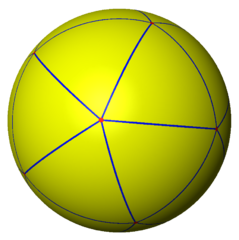
\includegraphics[scale=1]{Fig11}
\caption{A tiling of the elliptic plane.} 
\end{figure}

\begin{figure}[h]
\centering
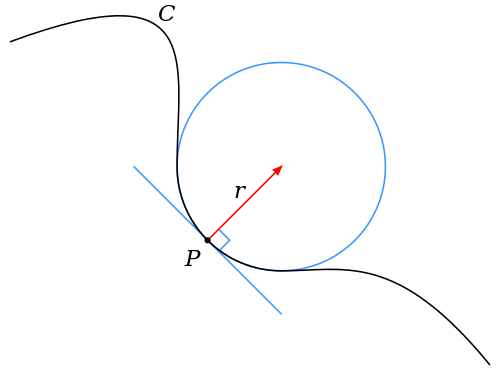
\includegraphics[width=0.5\textwidth]{Fig21}
\caption{A diagram of curvature at a point \(P\) with its "approximation circle" of radius \(r\).} 
\end{figure}

\begin{multicols}{2}

The curvature of a plane curve\footnote{ A plane curve can for our purposes be considered any line, wiggly or straight, drawn continuously on a surface.} at a specific point \(A\) can be considered intuitively as a measure of how effectively a tangent at \(A\) can be used to approximate the location of points just around \(A\) or how fast the tangent diverges from the actual curve as one moves away from \(A\). More rigourously, given any curve and a point \(A\) somewhere along it, there is a circle with a centre \(O\) on the line perpendicular to the tangent at \(A\) (called the \textit{normal}) with \(|OA| = r\) for some \(r\) (\(r\) is the radius). This is the best circle which approximates the curve for points close to \(A\)---an illustration of this concept can be seen in \textbf{Fig. 3.2}. We define \(\kappa\) to be the curvature, where \(\kappa = \frac{1}{r}\).

Using this, we can define Gaussian curvature, which is a way of measuring the intrinsic curvature of surfaces. Given a point \(A\) on a surface, consider the normal at \(A\) (here this is the perpendicular line to the \textit{tangent plane} at \(A\)) and then, further, consider all the planes that contain that normal. Each of the planes will intersect with a 1-dimensional cross-section of our surface, and so for each intersecting plane \(P_n\), we calculate the curvature of the corresponding 1-dimensional plane curve at \(A\), denoted \(\kappa_n\). Now, the \textit{Gaussian curvature} of \(A\) is defined to be the product of the maximum and minimum such \(\kappa_n\) (known as the \textit{principal curvatures} at the point \(A\)). So, let's stop to consider what the Gaussian curvature of various well-known surfaces looks like: 
\begin{itemize}
\item with a point on a plane, the curvature of a point on any plane-cross-section is 0, since the best circle which approximates a straight line has an infinitely large radius\footnote{In other words, \( \lim_{R \to \infty} \frac{1}{R} = 0\)}, so \(\kappa_{max}, \kappa_{min} = 0\), so the Gaussian curvature is 0; 
\item with a point on a cylinder, the curvature of the long straight axis is \(\kappa_{min}\) which is 0 for the same reason as on the plane and so regardless of \(\kappa_{max}\), its G. curvature is 0; 
\item with a point on a sphere, every plane-cross-section will be a circle of radius \(R\), meaning that \(\kappa_{min}, \kappa_{max} = \frac{1}{R}\) and so the G. curvature is \(\frac{1}{R^2}\) at every point.
\end{itemize}

\end{multicols}
 
\begin{figure}[h]
\centering
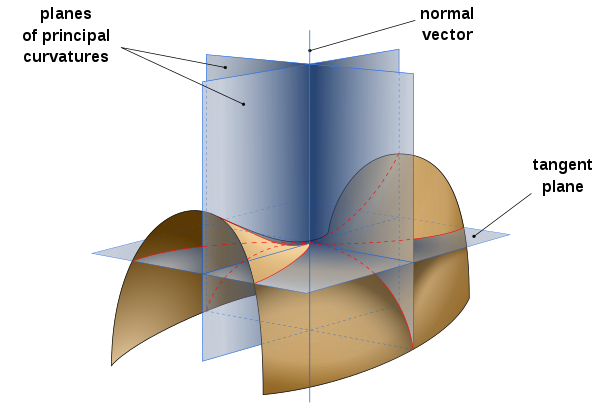
\includegraphics[width=0.5\textwidth]{Fig31}
\caption{A "saddle-surface".} 
\end{figure}

\begin{figure}[h]
\centering
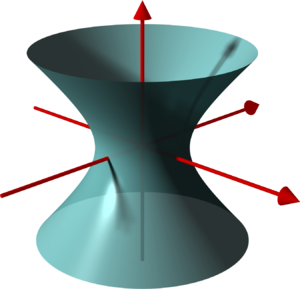
\includegraphics[scale=0.5]{Fig41}
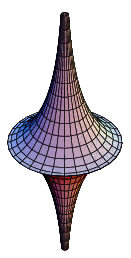
\includegraphics[scale=0.5]{Fig42}
\caption{A hyperboloid and a pseudosphere.} 
\end{figure}

\begin{multicols}{2}

What would a point of negative curvature on a surface look like? Consider \textbf{Fig. 3.3}, displaying a so-called "saddle-surface". At the centre of the saddle, the diagram displays the planes which intersect the surface at its principal curvatures---one of the cross-sections curves upwards in the direction of the normal and the other, 90\(^\circ\) to the first, curves downwards against the direction of the normal. The former would have some positive \(\kappa_{max}\) but since the other curves downwards from the normal, Gauss said it would be natural to assign the downwards curve a negative \(\kappa_{min}\) and so the Gaussian curvature (their product) would also be negative. The interesting question that Gauss asked after considering this was: what would a surface with constant negative curvature look like? After giving the problem some thought, one might come up with the surfaces shown in \textbf{Fig. 3.4}; one is a \textit{hyperboloid} (the surface of revolution of a hyperbola) and the other is called a \textit{pseudosphere}, discovered by Bolyai. Both have negative curvature at almost all of their points but neither have constant negative curvature.

In trying to understand the problem better, one can examine the geometric properties of such a surface, and what one discovers is that triangles have less than or equal to 180\(^\circ\) as their summed internal angles etc.---this is just a different description of the hyperbolic plane! Although Gauss never did gain much better insight into the nature of such a surface, he did prove the important \textit{Theorema Egregium} which says that by performing cutting, rotating, translating or bending operations on a surface, one sustains the same Gaussian curvature at every point; thus, Gaussian curvature is a defining "unalterable" property of a surface, showing clearly why one can't wrap a piece of paper around a sphere as easily as around a cylinder---the piece of paper has constant zero curvature, and the sphere has \(\frac{1}{R^2}\), and so to cover the sphere with paper, one would have to be able to stretch or otherwise fundamentally alter its nature. It also shows why rolling up a piece of paper into a cylinder makes it so much more rigid than when it was just flat: when you've rolled it up, you have created a positive curvature in one direction and so for the paper to retain its constant zero Gaussian curvature, it has to stay straight in the other direction...

The final piece of the puzzle came from the work of the prolific David Hilbert with \textit{Hilbert's Theorem}\footnote{It should be noted that this name, just like \textit{Euler's Theorem} in modular arithmetic, is completely ridiculous since the individual it's named after proved many hundreds of theorems and is commonly considered to be amongst the most important of mathematicians of the 19th and 20th centuries.}, which essentially proved that given an \(n\)-dimensional hyperbolic geometric space (as in, an \(n\)-space of constant negative curvature) there is no distance and angle-preserving way of putting it into an \(n\)-dimensional Euclidean space, certifying that this is a consistent and fundamentally distinct geometry.

\end{multicols}

\section{Schl\"{a}fli notation and tilings}

\begin{multicols}{2}

For those who read the first article in this series, you would have seen an introduction to some of the many combinatorial and geometric problems and properties of tilings of the Euclidean plane. It was suggested then that hyperbolic geometry sported a much greater collection of such tilings and now we shall see that such comments are quite justified and that, in some sense, most tilings are in fact hyperbolic. 

The \textit{Schl\"{a}fli symbol} \(\{x_2, x_1\}\) is a notation used to denote a tiling where there are \(x_1\) \(x_2\)-gons around a point. So, for example, the Schl\"{a}fli symbol \(\{4,4\}\) describes the classic square-lattice tiling on the Euclidean plane and \(\{3,5\}\) describes the tiling in \textbf{Fig. 3.1}. You might notice that this notation severely limits the number of tilings one can describe, since one can only notate those which use only 1 shape, and in which each vertex has the same number of polygons around it (these are known as the \textit{regular tilings}), but it is still useful. What symbols \(\{p,q\}\) are Euclidean?

Well, it can only be Euclidean if the sum of \(q\) of the internal angles of \(p\)-gons is 360\(^\circ\)---that is \(q(180^\circ-\frac{360^\circ}{p}) = 360^\circ\). This is equivalent to the statement that \((p-2)(q-2) = 4\). By graphing this line with one axis being \(p\) and the other \(q\), we get \textbf{Fig. 3.5}.

\end{multicols}

\begin{figure}[h]
\centering
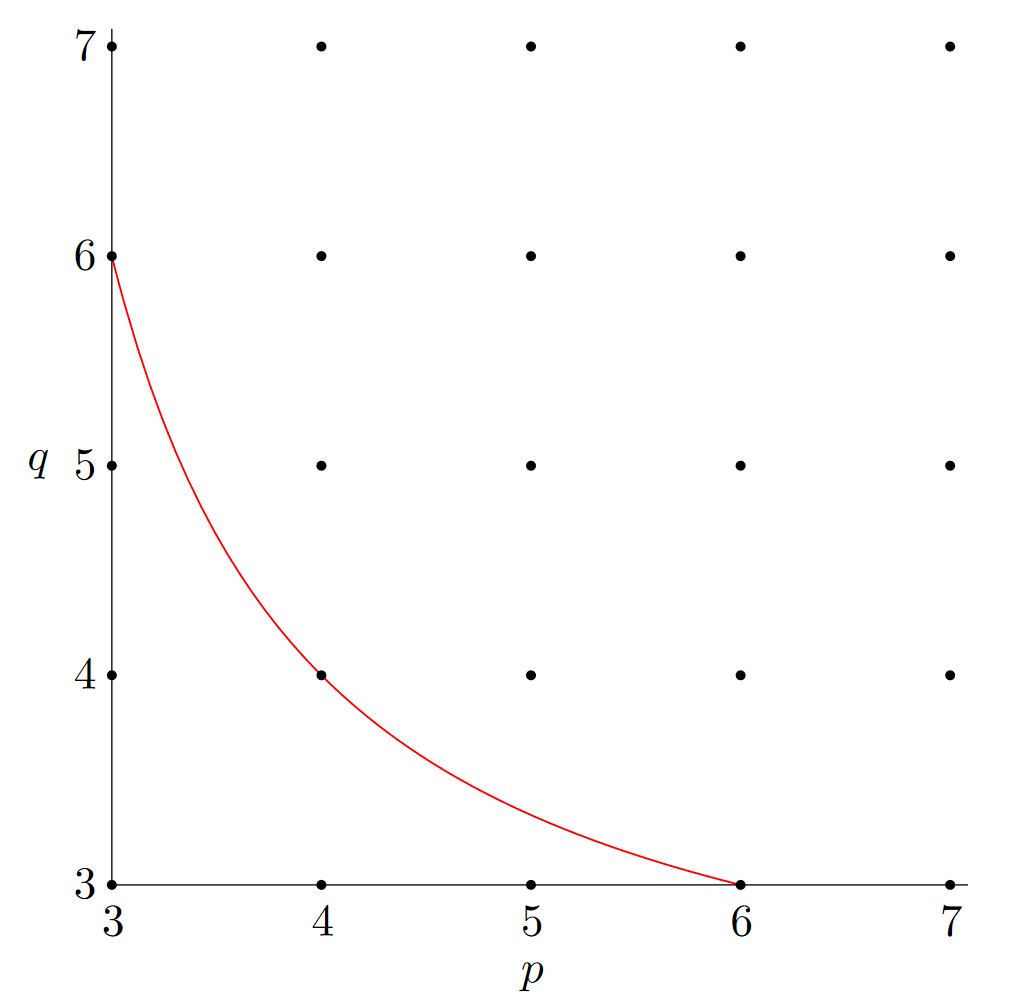
\includegraphics[width=0.5\textwidth]{Fig51}
\caption{A graph of the Euclidean tilings.} 
\end{figure}

\begin{multicols}{2}

This diagram is quite powerful in that it shows clearly the space of regular tilings in each geometry. Those on the line are Euclidean such as \(\{3,6\}\), those below the line are elliptic such as \(\{3,4\}\), and the infinity of those above it are \textit{all} hyperbolic! With so many, one would hope that there would be a way of visualising or creating images of these tilings---thanks to the work of Henri Poincar\'{e} and Felix Klein, you can look at visualisations of the hyperbolic plane.

Both of them act as a projection of the hyperbolic plane to the unit disk\footnote{The set of points on the Euclidean plane of distance less than or equal to 1 from \((0,0)\).} where the edge of the disk can be seen as the "edge at infinity" of the hyperbolic plane---although I will not mention the specifics of geometric constructions or calculations with them in this article, it should be clear that distances in the disk going out from the centre become increasingly large for the corresponding hyperbolic figures. In the Poincar\'{e} disk model, lines are represented by circle arcs drawn in the disk which are orthogonal to the disk's edge and the model represents angles accurately (this property of a mapping from one space to another is known as \textit{conformality}). In the Klein model, conformality is lost with the benefit that lines are drawn straight here. The same \(\{7,3\}\) tiling is represented using the two models in \textbf{Fig. 3.6}---though in general the images I will use in this article and any articles involving hyperbolic space in the future will use the Poincar\'{e} disk model due to its angle preserving nature.

Another incredible object that can exist in hyperbolic tilings is the \textit{apeirogon} or \(\infty\)-gon (a polygon with an infinite number of sides). In Euclidean tilings the only way it can be represented is in "degenerate"\footnote{The word \textit{degenerate} is used in mathematics to describe objects or situations which technically fulfill specific requirements but are so devoid of structure or meaning that they are worthless to study. Another example of a degenerate object would be the 2-sided or 1-sided polygons (which, on the Euclidean plane, are just straight lines).} tilings, such as can be found in \textbf{Fig. 3.7}, where the "sides" of the polygon are just an infinitely long line separated by dots denoting vertices at regular intervals. The image can be seen as a tiling of the Euclidean plane by 2 apeirogons.

However, hyperbolic space is sufficiently curved and "large" that apeirogons can exist as discrete shapes surrounded by other polygons and that, equally, there can be tilings with an infinite number of polygons around each vertex, such as those shown in \textbf{Fig. 3.8}! In this case, all the vertices of the tiling are actually points at the edge of the disk and thus at infinity, known as \textit{ideal points}.

\end{multicols}

\begin{figure}[h]
\centering
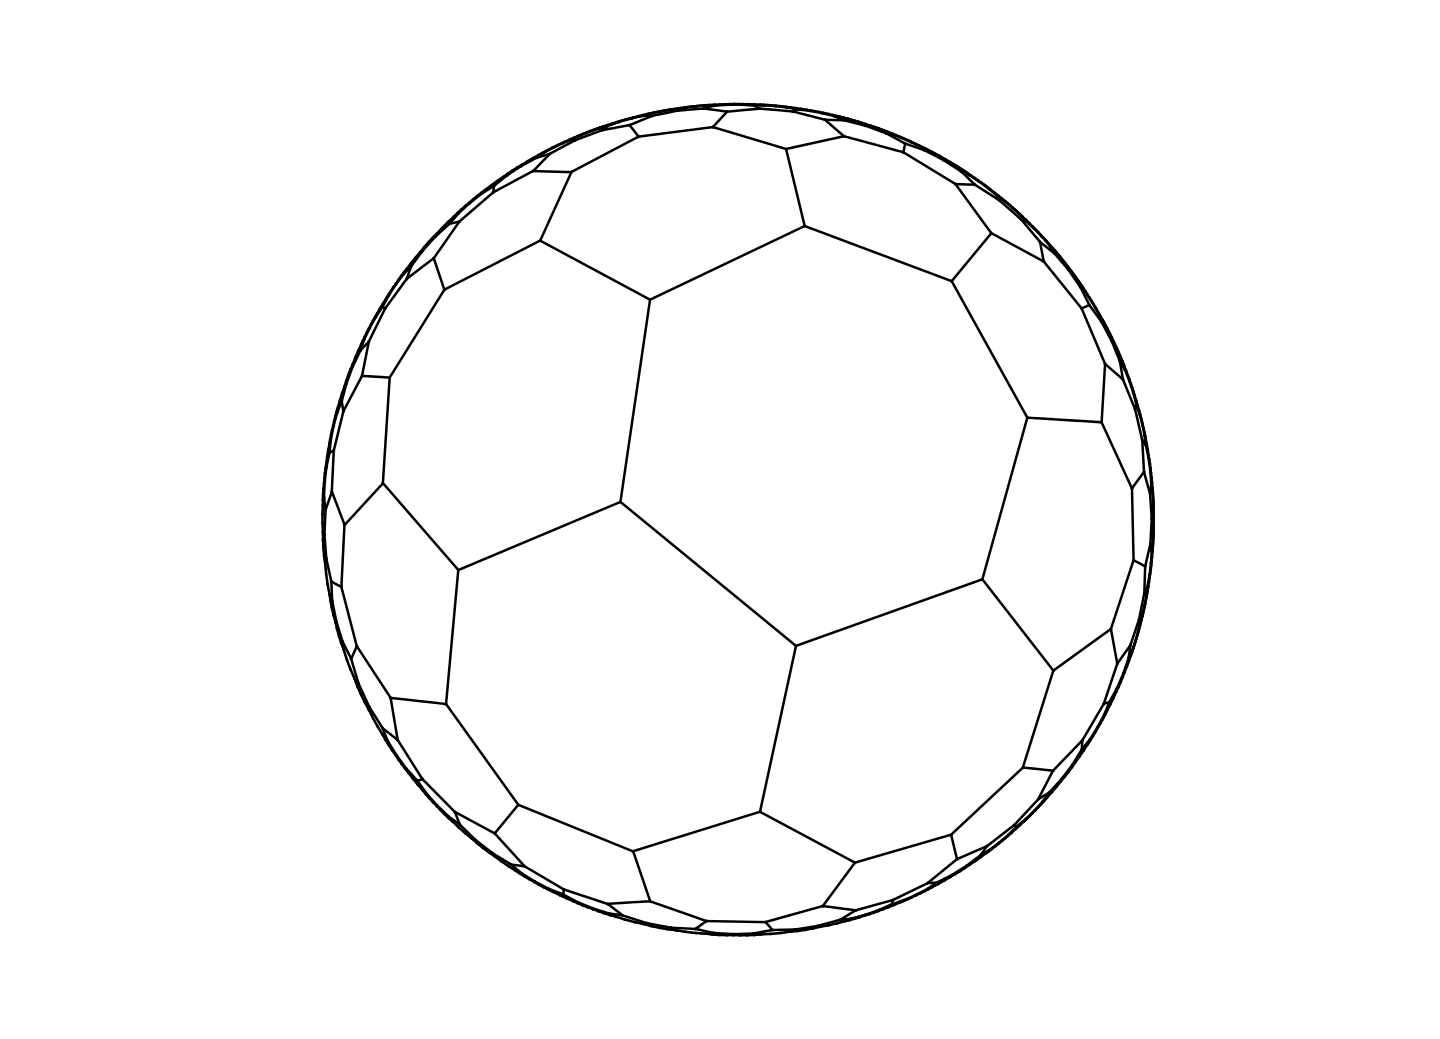
\includegraphics[width=0.3\textwidth]{Fig61}
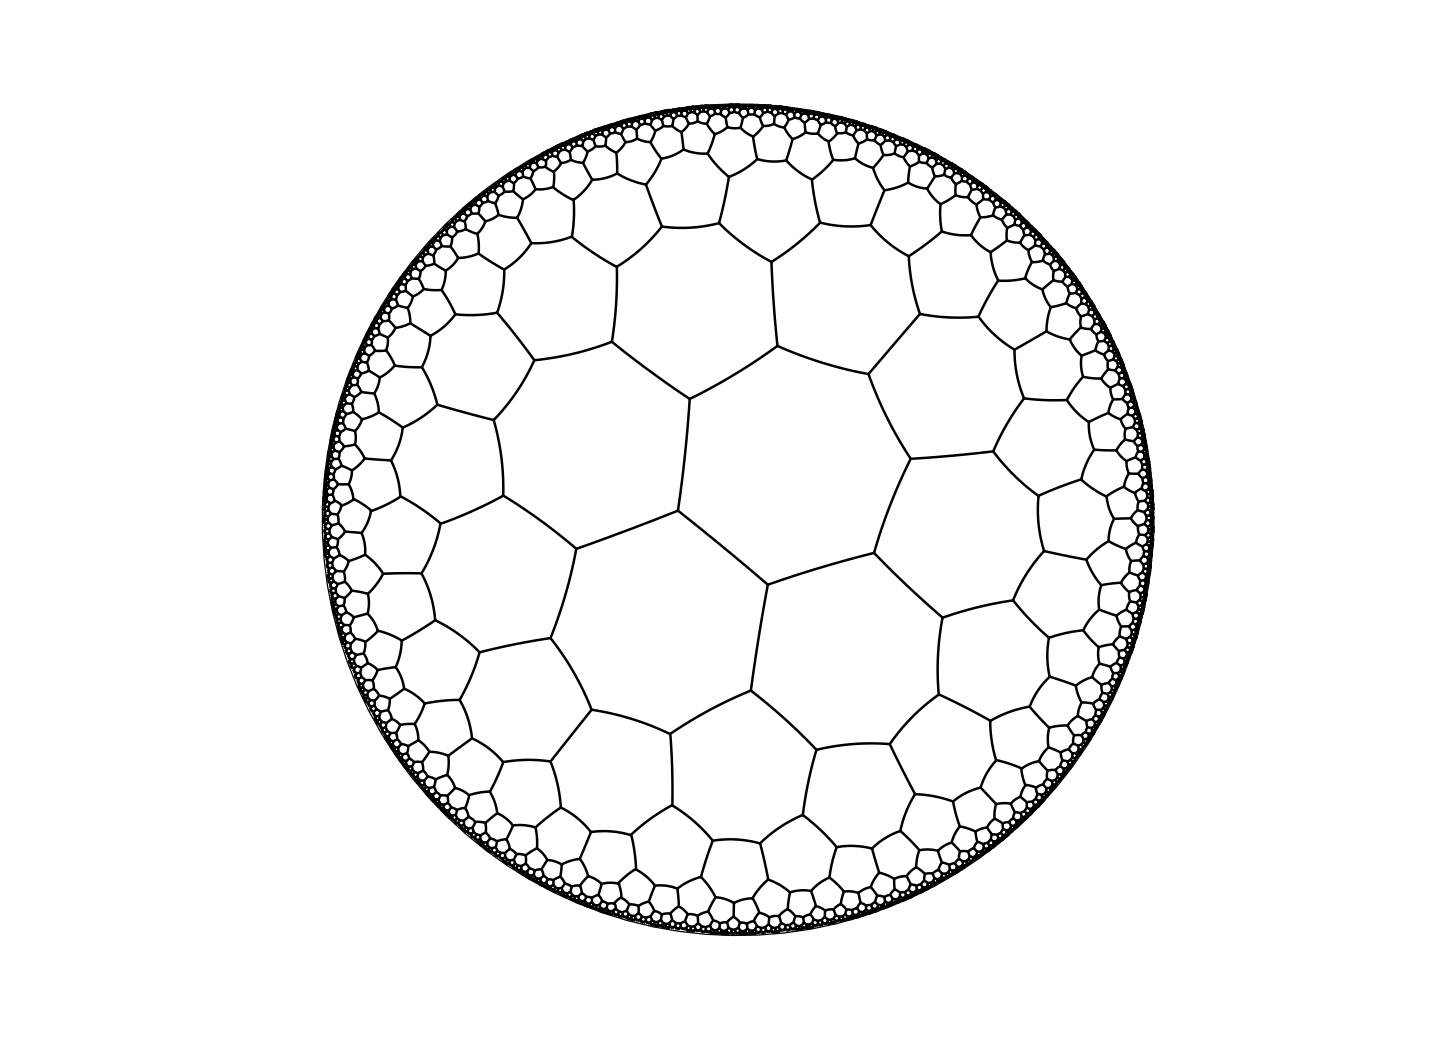
\includegraphics[width=0.3\textwidth]{Fig62}
\caption{A \(\{7,3\}\) tiling projected into the Klein Model and the Poincare Model.} 
\end{figure}

\begin{figure}[h]
\centering

\includegraphics[width=0.5\textwidth]{Fig71}
\caption{A \(\{\infty,2\}\) tiling.} 
\end{figure}

\begin{figure}[h]
\centering
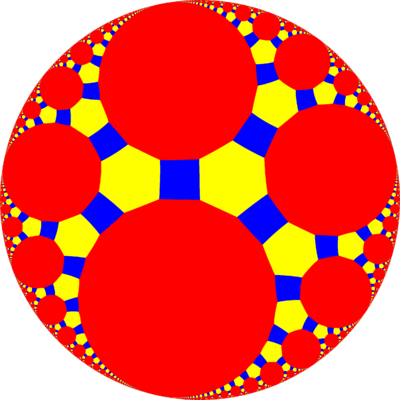
\includegraphics[width=0.25\textwidth]{Fig81}

\includegraphics[width=0.25\textwidth]{Fig82}
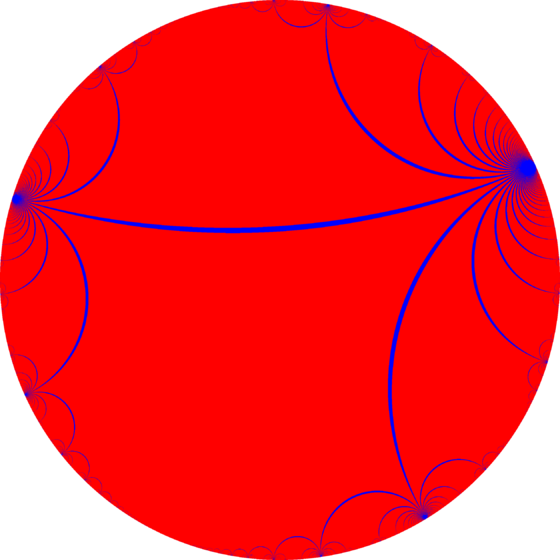
\includegraphics[width=0.25\textwidth]{Fig83}
\caption{A tiling of apeirogons with squares and hexagons, the \(\{3,\infty\}\) tiling and the \(\{\infty,\infty\}\) tiling.} 
\end{figure}

\section{Higher-dimensional Hyperbolic Space, Horocycles and beyond...}

\begin{multicols}{2}

Hyperbolic geometry becomes even more complicated in 3-space, or 4 or further! In order to investigate these spaces we need to understand the extended definition of the Schl\"{a}fli symbol and learn about \textit{horocycles}. In general, the Schl\"{a}fli symbol \(\{x_n, x_{n-1},...,x_2,x_1\}\) denotes \(x_1\) copies of \(\{x_n, x_{n-1},...,x_2\}\) around each vertex---this allows us to talk about regular \textit{honeycombs} of arbitrary dimensions! You can see some examples of different cube-based polyhedron packings in \textbf{Fig. 3.9}, going from the elliptic to the hyperbolic (represented here by the Poincar\'{e} \textit{sphere} model).

Most interesting, however, is the next in the series, namely \(\{4,3,6\}\), whose vertices are purely ideal. To see why \(\{4,3,6\}\) would suddenly have only ideal vertices while all its predecessors have none, we can look at its \textit{dual honeycomb}. The dual of a honeycomb is formed by taking the geometric centres of every face of every polyhedron involved and drawing lines between those that are adjacent to each other (as in, those which are part of a common polyhedron). 2D examples are easier to visualise at first, so let's take a look at some: in \textbf{Fig. 3.10}, we see two diagrams, one showing how the square tiling \(\{4,4\}\) is self-dual, where the original tiling is in blue and the dual is in red, the second showing how the dual of the cube (corresponding to the Schl\"{a}fli symbol \(\{4,3\}\)) is the octahedron (with symbol \(\{3,4\}\). Can you spot a pattern here?

The dual of a geometric structure defined by the symbol \(\{x_n, x_{n-1},...,x_2,x_1\}\) is \(\{x_1, x_2,...,x_{n-1},x_n\}\)! Can you think why this is? 

It allows us to see that the dual of \(\{4,3,6\}\) is \(\{6,3,4\}\), which can be interpreted as having 4 of the polyhedron \(\{6,3\}\) around a point... except that \(\{6,3\}\) defines the normal Euclidean hexagonal tiling of hexagons... Remarkably, hyperbolic space is so curved that it permits Euclidean tilings as infinite-sided polyhedra where the plane curves in on itself and becomes a form of hyperbolic ball---such an object is known as a \textit{horocycle}\footnote{The official definition of a horocycle is a curve in hyperbolic space with the property that all lines intersecting it orthogonally tend to the same ideal point, but for our purposes the above commentary will suffice.} and to me it's simply astounding that such an object could exist. Consequently, since the definition of a dual honeycomb \(B\) of a honeycomb \(A\) requires that the number of faces of the polyhedra in \(B\) is the same as the number of the edges going into the vertices of \(A\), it follows that there are infinite number of lines going into the vertices of \(\{4,3,6\}\) and thus its vertices are ideal.

\end{multicols}

\begin{figure}[h]
	\centering
	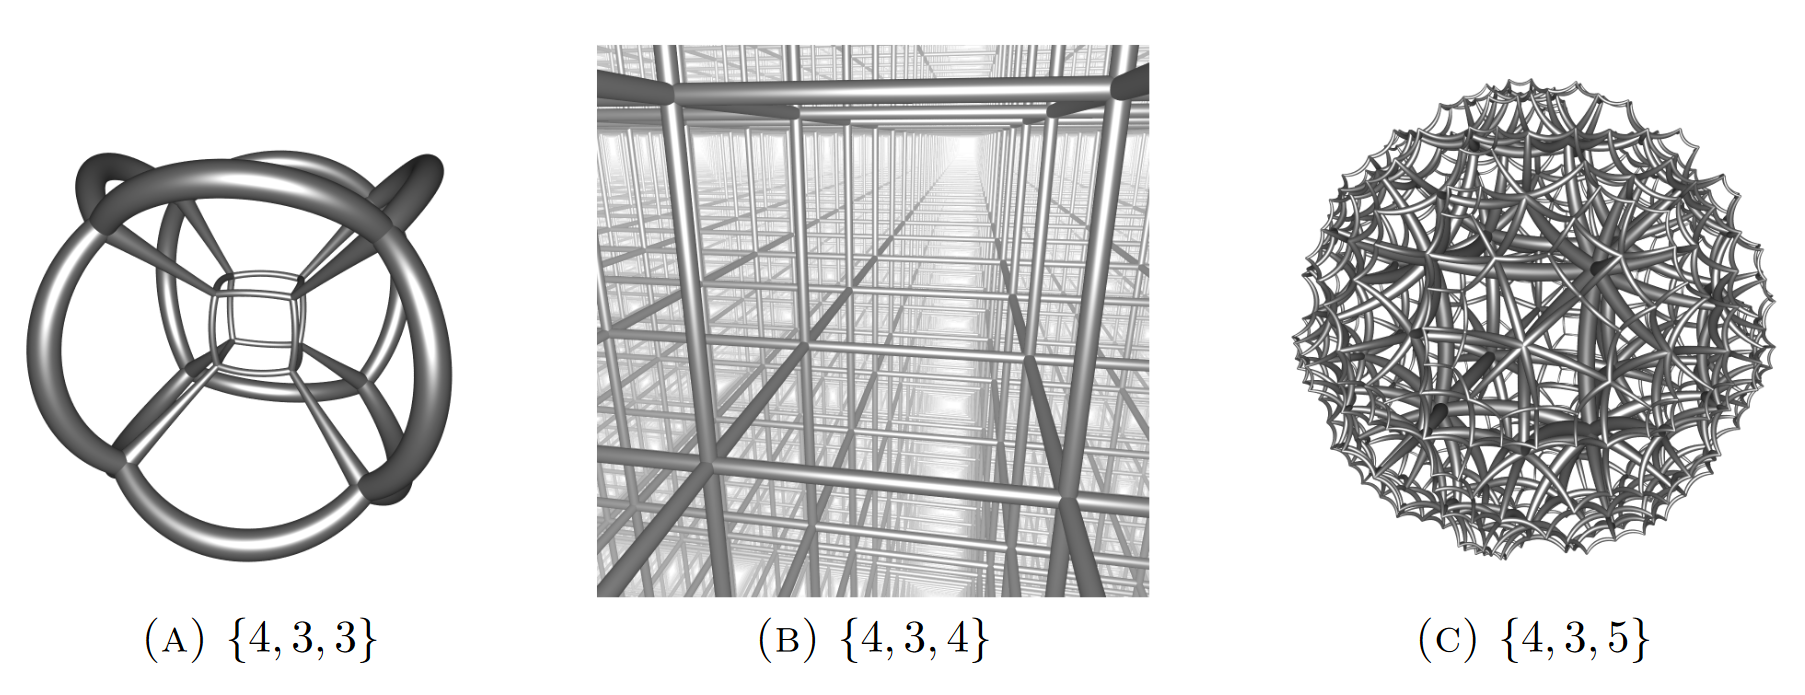
\includegraphics[width=0.5\textwidth]{Fig91}
	\caption{A series of three poyhedron packings in different spaces with their respective Schl\"{a}fli symbols.} 
\end{figure}

\begin{figure}[h]
	\centering
	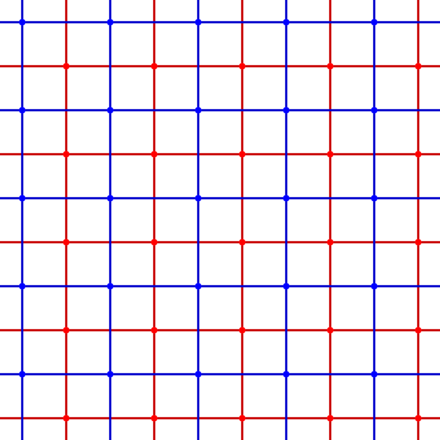
\includegraphics[width=0.4\textwidth]{Fig101}
	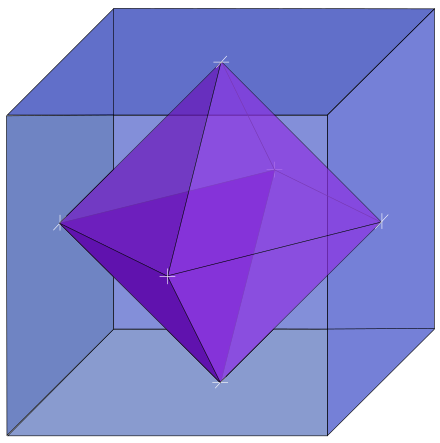
\includegraphics[width=0.4\textwidth]{Fig102}
	\caption{The duals of \(\{4,4\}\) and \(\{4,3\}\).} 
\end{figure}

\begin{multicols}{2}

Modern-day geometry is even stranger than much of what we have talked about here. Instead of studying simply the Euclidean plane, one studies general \textit{affine planes}, for which Euclid's first and fifth axiom hold along with the requirement:

\begin{itemize}
\item There are four points such that no line is incident with more than two of them.
\end{itemize}

and instead of studying the elliptic plane, mathematicians examine \textit{projective planes}, in which Euclid's first axiom holds, there are no parallel lines and the above requirement holds. Further, both of the planes just mentioned can be realised using any number system (or for those who know some abstract algebra, any \textit{field})---for example, one can create the affamed Complex Projective Plane by considering \(\mathbb{C}^3\) and then calling the set of lines going through the origin "points" or, equivalently, saying that two points \((x_1,x_2,x_3)\) and \((y_1,y_2,y_3)\), with \(x_n,y_n \in \mathbb{C}\), are "the same" if there is some complex number \(z\) so that \((zx_1,zx_2,zx_3) = (y_1,y_2,y_3)\). In this odd world where points' coordinates are described using complex numbers and lines are planes intersecting the origin, one can have many objects that we could never have in our own geometries such as the 3-dimensional surfaces known as \textit{3-folds}---these exist in Complex Projective 4-space and often have so many rotational or complex symmetries that they simply have no analogue in our universe.

For those of you that have enjoyed this article, you may wish to read up on \textit{differential geometry}, in which \textit{Riemannian manifolds}, a generalisation of traditional geometric surfaces to any number of dimensions and which only have the requirement that areas "near" each point act analogously to Euclidean space\footnote{The official definition is a \textit{topological space} which has a neighbourhood associated with every point that is \textit{homeomorphic} to some Euclidean \(n\)-space equipped with a useful object for measuring distances known as a \textit{Riemannian metric}, but that's for extra reading!}---it has really allowed mathematicians to better grasp what "spaces" \textit{are} and the various properties that they could have... Riemann himself was the top student of Gauss and formulated the above concepts after being introduced to Gaussian curvature by his mentor! So, for further reading, look up:

\begin{itemize}
\item The notion of a \textit{field} in abstract algebra and how they are used in the definitions of \textit{projective} and \textit{affine planes}.
\item \textit{Topological} spaces.
\item \textit{Uniform tilings} of the hyperbolic plane; there's an excellent Wikipedia page on this that contains many more images than in this article!
\item \textit{Riemannian} geometry; although you shouldn't expect to pick this up immediately, since it is a complex subject, true understanding of this should make General Relativity easy to read!
\item Hypercycles and the actual definition of horocycles
\item \textbf{Definitely}, if nothing else, go to "h3.hypernom.com" and try and use your arrow keys and WASD to move around---it's a simulator of hyperbolic 3-space from within the Poincar\'{e} sphere.
\end{itemize}

\end{multicols}

\section{Challenge V}

\begin{multicols}{2}

And now, as per usual the challenge with a relatively simple first part and a second part that I know \textit{no} good solutions to---if you have solutions to either of these, please email either \textbf{Isky Mathews} or \textbf{Benedict Randall Shaw} with them!

\begin{itemize}
\item What structure does the symbol \(\{5,3,4\}\) describe?
\item Can you come up with a notation for tilings, polyhedra and honeycombs which works for \textit{non-regular}, \textit{non-vertex transitive} structures?
\end{itemize}

\end{multicols}

\chapter{A Reintroduction to Areal Co\"ordinates}

\textbf{Benedict Randall Shaw}

\begin{multicols}{2}

Several issues ago, an article was published in this publication with the title \say{An Introduction to Areal Co\"ordinates}. Regrettably, having revisited this article, it seems to have been below the usual standard, and worryingly cursory. However, the topic itself is of use and interest; thus, this article is intended to do that which the original failed to, viz. introduce the reader to areal co\"ordinates.

This article is aimed at those who wish to do vaguely well in olympiads, but find themselves unable to do geometry by Euclidean (normal) methods. While most olympiad questions are designed to be done by such methods, there exist other ways of doing geometry problems. Areal co\"ordinates are an example of such a method; they constitute a co\"ordinate system, in the same way that Cartesian co\"ordinates (those with which most people are most familiar) are a co\"ordinate system. They are not always successful, but tend to be useful in problems where a triangle is the central object involved.

In order to become competent with mathematic concepts, it is helpful to practise; so, throughout this article I shall leave questions that can be done by those wishing to become competent.

\fbox{Such questions will be placed in boxes, thus.}

\end{multicols}
\section{Definitions}
\begin{multicols}{2}

We say that a point anywhere in the plane \(P\) has co\"ordinates \((x,y,z)\) with respect to a triangle \(\triangle{}ABC\) iff \[(x,y,z)=\left(\frac{[PBC]}{[ABC]},\frac{[APC]}{[ABC]},\frac{[ABP]}{[ABC]}\right)\] where \([DEF]\), for some triangle \(DEF\), is the area of \(\triangle{}DEF\).

\end{multicols}

\begin{figure}[h]
	\centering
	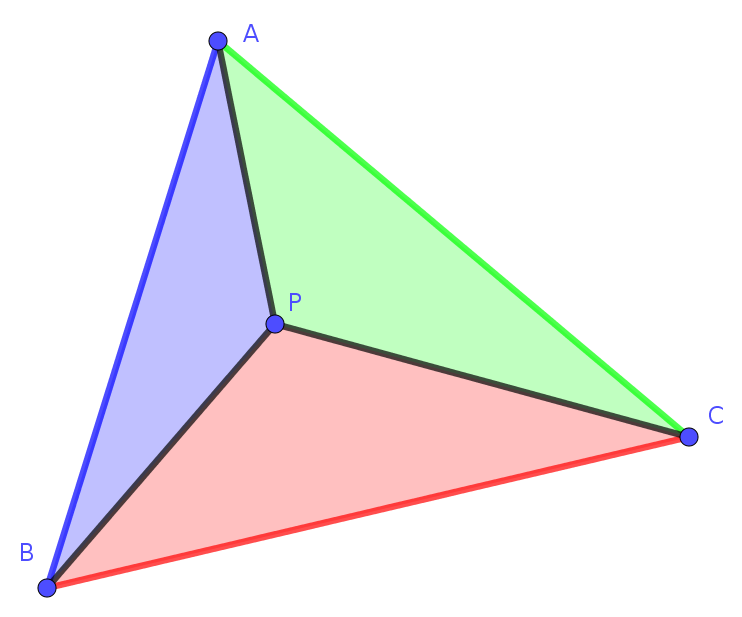
\includegraphics[width=0.5\linewidth]{def-areas}
	\caption{A point \(P\), with respect to \(\triangle{}ABC\).}
	\label{def-areas}
\end{figure}

\begin{multicols}{2}

Note that \(x+y+z=1\) is thus always true, as clearly \([PBC]+[APC]+[ABP]\). We thus have a rigorously defined unique set of co\"ordinates for all points within the triangle. But what about those outside the triangle? First, we must define directed areas. When we name a triangle, convention says that we label its points anticlockwise. We therefore say that \([ABC]\) is positive if \(A,B,C\) are in order going anticlockwise around \(\triangle{}ABC\), and negative if the points are in order going clockwise. (If the points \(A,B,C\) are in a straight line, then \([ABC]\) is obviously zero.) We now have a distinct set of co\"ordinate for all points in the plane. \fbox{Prove this.}

An equivalent definition exists with vectors. For any arbitrary point \(O\) in the plane, point \(P\) has co\"ordinates \((x,y,z)\) with respect to \(\triangle{}ABC\) iff \(\overrightarrow{OP}=x\overrightarrow{OA}+y\overrightarrow{OB}+z\overrightarrow{OC}\) and \(x+y+z=1\). It does not matter where we choose \(O\); we get the same set of co\"ordinates for \(P\) whereever \(O\) is. \fbox{Prove this.}

\begin{center}
\fbox{\parbox{0.96\linewidth}{Prove that these two definitions, in terms of areas and vectors are equivalent; that is to say, all points have the same co\"ordinates under both definitions.}}\\
\end{center}

For the physically minded, there is also yet another definition; \((x,y,z)\) is the point that is the centre of mass when one places masses \(x,y,z\) at points \(A,B,C\) respectively, such that \(x+y+z=1\). Note that we allow negative masses.

It is clear that \(A,B,C\) have co\"ordinates \((1,0,0),(0,1,0),(0,0,1)\) respectively; from consideration of the definition involving areas, one can see that a point is within the triangle if and only iff all its co\"ordinates are positive.

Often we don't care about the constraint \(x+y+z=1\), and so we relax it; there is no single standard notation for this of which this correspondent is aware, so in this article, we shall use \((x,y,z)^*\) to denote \((\frac{x}{x+y+z},\frac{y}{x+y+z},\frac{z}{x+y+z})\). These are sometimes referred to as unnormalised co\"ordinates.

\end{multicols}
\section{Triangle centres}
\begin{multicols}{2}

Triangles do not have an obviously defined centre; as a result, there are numerous points known as \textit{triangle centres}, to the point where they have an encyclop\ae{}dia, which at time of writing contains 15888 centres, and is imaginatively named the \textit{Encyclopedia of Triangle Centers} (it is admittedly American). Needless to say, most of these are completely useless; however, the centres are loosely sorted by importance, and the encyclop\ae{}dia gives the areal co\"ordinates of the earlier centres, although it calls them barycentrics. Here are some important centres, and their co\"ordinates with respect to \(\triangle{}ABC\) (when they are the centres of the \(\triangle{}ABC\)). \(a,b,c\) refer to the lengths of sides \(BC,CA,AB\) respectively, and \(A,B,C\) refer to angles \(\angle{}CAB,\angle{}ABC,\angle{}BCA\) respectively.

\paragraph{Incentre} This is the centre of the incircle (the circle within the triangle tangent to all three sides) and also the intersection of the internal angle bisectors of the triangle; it has co\"ordinates \((a,b,c)^*\).

\paragraph{Centroid} This is the intersection of the medians of the triangle (the lines from vertices of the triangle to midpoints of the opposing sides); it has co\"ordinates \((1,1,1)^*\).

\paragraph{Circumcentre} This is the centre of the circle passing through all three vertices of the triangle, and the intersection of the perpendicular bisectors of the sides; it has co\"ordinates \((\sin{}2A,\sin{}2B,\sin{}2C)^*\).

\paragraph{Orthocentre} This is the intersection of the altitudes of the triangle (the perpendiculars from the vertices to the opposing sides); it has co\"ordinates \((\tan{}A,\tan{}B,\tan{}C)^*\).

\begin{center}
\fbox{\parbox{0.96\linewidth}{Prove that these are the correct co\"ordinates for the four triangle centres mentioned, whatever the triangle.}}
\end{center}

These four points are often sufficient; there are many theorems involving them, and they appear frequently in olympiads. Other points, and their co\"ordinates, can be found in the \textit{Encyclopedia of Triangle Centers}.
\end{multicols}
\section{Lines}
\begin{multicols}{2}
In the same way that the general equation for a line in Cartesian co\"ordinates is \(lx+my+c=0\) (where \(l,m,c\) are constants that are not all zero), the general equation for a line in areal co\"ordinates is \(lx+my+nz=0\) (where \(l,m,n\) are constants that are not all zero), in addition to the standard \(x+y+z=1\) required by areals. Note that this equation still works if we relax the \(x+y+z=1\) constraint and use unnormalised co\"ordinates, as scaling \(lx+my+nz\) by a constant still gives 0 for a point that is on the line.

The equation of a line through two points \((x_p,y_p,z_p)\) and \((x_q,y_q,z_q)\) is expressed most readably with a matrix determinant. For those unaware of them, matrices are rectangular arrays of numbers. We define the determinant (written with vertical lines around a matrix) of a two by two matrix thus---
\[\begin{vmatrix}a&b\\c&d\end{vmatrix}\equiv{}ad-bc\]

We define the determinant of a three by three matrix thus---
\[\begin{vmatrix}a&b&c\\d&e&f\\g&h&i\end{vmatrix}\equiv{}g\begin{vmatrix}b&c\\e&f\end{vmatrix}+h\begin{vmatrix}c&a\\f&d\end{vmatrix}+i\begin{vmatrix}a&b\\d&e\end{vmatrix}\]

The equation for a line through points \((x_p,y_p,z_p)\) and \((x_q,y_q,z_q)\) is given by this equation---
\[\begin{vmatrix}x_p&y_p&z_p\\x_q&y_q&z_q\\x&y&z\end{vmatrix}=0\]

Note that a line \(lx+my+nz=0\) passes through \(A\) iff \(l=0\), \(B\) iff \(m=0\), and \(C\) iff \(n=0\). This is fairly apparent from consideration of the co\"ordinates of the vertices. Note that if two of the co\"efficients are zero, then the line must be one of the sides of \(\triangle{}ABC\). \fbox{Prove this.}
\end{multicols}
\clearpage
\section{Areas}
\begin{multicols}{2}
For points \(P,Q,R\) with co\"ordinates  \((x_p,y_p,z_p),(x_q,y_q,z_q),\\(x_r,y_r,z_r)\), the area of \(\triangle{}PQR\) (which we denote \([PQR]\)) is given by this formula---

\[
[PQR]=[ABC]\begin{vmatrix}x_p&y_p&z_p\\x_q&y_q&z_q\\x_r&y_r&z_r\end{vmatrix}
\]

This should sound reasonable, based on the determinant definition of a line through two points; it is clear that \([PQR]=0\) iff \(P,Q,R\) are collinear, so \(R\) lies on line \(PQ\) iff the determinant has value zero.

Note that this formula clearly does not work for unnormalised co\"ordinates.

This is often enough to solve olympiad problems, along with some trigonometric competence.
\end{multicols}
\section{Circles}
\begin{multicols}{2}
Where \(a,b,c=|BC|,|CA|,|AB|\), the \textit{circumcircle} of \(\triangle{}ABC\) (the circle going through all three points \(A,B,C\)) is given by the equation \(a^2yz+b^2zx+c^2xy=0\). In fact, the general equation for a circle is given by \(a^2yz+b^2zx+c^2xy+lx+my+nz=0\), when we are using the constraint \(x+y+z=1\). If we relax that and use unnormalised co\"ordinates, we have the slightly more complex equation \(a^2yz+b^2zx+c^2xy+(x+y+z)(lx+my+nz)=0\).

For a circle in the plane passing through three points, we can find its equation by substituting the three points into the general equation and finding \(l,m,n\).
\end{multicols}
\section{Vectors \& Distances}
\begin{multicols}{2}
For those who are unaware of what a vector is, a vector denotes a specific geometric translation; that is to say, it denotes a way to move a point to another. For example, in Cartesian co\"ordinates, \[\begin{bmatrix}3\\-2\end{bmatrix}\] is the vector that denotes moving a point or other object to the right by three units and down by two units; that is to say, it is the vector that would move \((0,0)\) to \((3,-2)\). In Cartesian co\"ordinates, the vector that would take \((x_p,y_p)\) to \((x_q,y_q)\) is  \[\begin{bmatrix}x_q-x_p\\y_q-y_p\end{bmatrix}\]
\textsl{}
In Cartesian co\"ordinates, we notate vectors differently to points, as there is no way to tell them apart if we write them the same way. In areals, this is not necessary, as will become clear. The vector taking \((x_p,y_p,z_p)\) to \((x_q,y_q,z_q)\) is \((x_q-x_p,y_q-y_p,z_q-z_p)\). We need not write the vector as a column, because the sum of the values in a vector is 0, as it is the sum of the co\"ordinates of one point minus the sum of those of another. It is thus easy to differentiate vectors and points. Note that when working with vectors in areals, we cannot use unnormalised co\"ordinates.

The length of a given line segment \(PQ\), where the vector taking \(P\) to \(Q\) (or vice versa) is \((u,v,w)\), can be found from this equation--- \[-PQ^2=a^2vw+b^2wu+c^2uv\]
which is reminiscent of the formula for circles, which should seem fairly natural given the usual definition of a circle as the set of all points which are a given distance from the centre.
\end{multicols}
\section{Disclaimer}
\begin{multicols}{2}
Ideally, one ought not to use areals, as the vast majority of geometric problems have neater, more satisfying, and easier solutions using standard Euclidean methods. However, if one is unable to use those effectively for some reason, and has tried and failed to rectify this, then areals are a possible alternative; one must, however, practise using them if one wishes to use them properly and efficiently. Note that there exist other ways of doing geometry aside from areals and Euclidean methods, including but not limited to vectors, trigonometry, complex numbers, and (although this is not recommended, and is usually unhelpful) origami.
\end{multicols}

\chapter{On Thermoacoustic Refrigeration}

\hspace{\fill}\textbf{Benedict Randall Shaw}'s notes on \textbf{James Tett}'s lecture.

\begin{multicols}{2}
	
These notes are part of an ongoing series of lecture reviews. To increase ease of comprehension and concision, they are not written using indirect or direct speech; rather, that which was said is simply replicated. \textit{The Librarian} does not endorse the content of any particular lecture.

Commentary, where provided, will be in \textbf{bold}. However, in these notes, \textbf{terms in bold} are to be defined immediately after; we use this convention here temporarily, and it may not be repeated.

\paragraph{Thermoacoustics} This should be fairly intelligible to anyone with a non-zero history of dealing with English words; being a combination of the prefix \say{thermo-}, meaning \say{relating to heat}, and \say{acoustics}, meaning \say{relating to sound}. The rough meaning of thermoacoustics should therefore be fairly apparent.

\paragraph{Sound} As anyone who has paid any attention through Fifth Form Physics will probably know, sound is composed of compressions and rarefactions of the medium through which the sound is travelling. However, Gay-Lussac's law tells us that, for a given mass and constant volume of an ideal gas, the pressure of said gas is directly proportional to its temperature in Kelvin. It therefore follows that, as sound is composed of oscillations in pressure, it must also be composed of oscillations in temperature. This is crucial to thermoacoustic refrigeration, as we shall go on to see.

\paragraph{Standing wave} A standing wave is a wave with a phase velocity of zero; that is to say, the peaks of the wave do not move spatially; rather, they simply oscillate in place. They are produced when two waves of equal amplitude, travelling in opposite directions, meet and overlap.

\paragraph{Refrigerator} While we commonly think of a refrigerator simply as being an appliance that makes an area cold, it does not do this by magic. Rather, what a refrigerator does is that it moves heat from one area to another, thus making the former colder and the latter warmer. Traditionally, the area made warmer is just that in which the refrigerator is.

One induces a standing wave of sound within a device called a resonator, which is essentially a long tube with some apparatus in, not by independently producing two waves of sound, but by producing one ordinary wave of sound using a loudspeaker at one end, and having the sound wave produced by it hit a hard surface at the other, which causes the wave to reflect back and overlap with itself, thus producing a standing wave. Note that being a sound wave, it therefore intrinsically involves oscillations in temperature and pressure.

The sound must be travelling through some medium; this is known as the working fluid (usually gaseous). Note that packets of the fluid expand when warm and compress when cold. As the temperature is oscillating in places due to the standing wave, there are therefore packets of air which become hot, and so expand and release heat, move forward, become cold, and so compress and absorb heat, move back again, and then repeat. This means that the packets of air absorb heat in one area and release it in another, and thus induce a temperature gradient in the surface to/from which they are releasing/absorbing heat.

To maximise this surface area, we use an item called a stack, which consists of many parallel channels. The standing wave therefore makes one end hot and one end cold; to use this, we put a microchannel heat exchanger at either end, which conducts heat to the cold end and away from the hot end. These heat exchangers have no moving parts.

We therefore have a mechanism that moves heat from one place to another, which is what we wanted.

\paragraph{Loudspeaker} We need the loudspeaker to be sufficiently sonorous to produce a wave of 180--200dB.

\paragraph{Working fluid} We want the working fluid to have a low viscosity to avoid inefficiency from friction, a high specific heat capacity to aid transfer of energy, and a thermoconductivity that is not too high, lest the temperature difference in parts of the fluid decrease as a result of heat moving from hotter areas to colder, but not too low, in order that heat may be absorbed from and released to the stack.

\paragraph{Stack} We want the stack to have a high surface area, to aid the transfer of heat between it and the fluid. We also want it to have a high specific heat capacity and a low conductivity, in order that the temperature gradient remains in place; that is to say, in order that the heat stays where we put it using our standing wave.

Thermoacoustic refrigerators have a number of advantages over those currently in household use, which have numerous problems: sliding seals are used, and so whatever manufacturers do, a small amount of refrigerant (the liquid used in the mechanism) will leak; they use a lot of power; and refrigerants themselves are nasty chemicals, often being flammable and toxic, and being harmful for the environment.

Thermoacoustic refrigerators avoid these problems to a large extent. The working fluid need not be toxic, and in fact can be a gas such as nitrogen, which forms \(78\%\) of the air and is non-toxic and inert (thus leakage does not matter); they are sufficiently efficient that they are used in space and by navies; and they only have one moving part (the loudspeaker), and so don't leak things.

At the moment, thermoacoustic fridges are expensive, as certain parts, such as the alternator required by the loudspeaker, are uncommon. However, they are starting to be used by the civilian population; for example, \(40\%\) of \textit{Ben and Jerry's} stores now use thermoacoustic refrigerators.
\end{multicols}

\chapter{How far do Isocrates and Plato agree about the teaching of rhetoric?}

\textbf{Benedict Mee}

\begin{multicols}{2}

By 387 BC, Plato had founded his famous Academy in Athens.\footnote{\textsuperscript{}
	Benoit, \emph{Isocrates and Plato on Rhetoric and Rhetorical
		Education}, 1991} Less well known today is another school, established
a few years earlier, probably around 392 BC, by Isocrates.\footnote{\textsuperscript{}
	Plutarch, \emph{Lives of Ten Orators}} While one of these teachers and
his school remain renowned even today, the other has faded into relative
obscurity. But it was not always so. Dionysius of Halicarnassus praised
Isocrates as `outstanding among the famous men of his day and the
teacher of the most eminent men in Athens and Greece'.\footnote{\textsuperscript{}
	Dionysius of Halicarnassus, \emph{Isocrates}} To Cicero, Isocrates was
`master of all rhetoricians'; in the eyes of Quintilian `we owe the
greatest orators to the school of Isocrates'.\footnote{\textsuperscript{}
	Cicero, \emph{De Oratore}; Quintilian, \emph{Institutio Oratoria}} By
the mid fourth century BC, Plato's Academy and Isocrates' school were
the two most prominent educational institutions in Athens.\footnote{\textsuperscript{}
	Grote, \emph{Plato and Other Companions of Socrates, 1867}} When
Plato's pupil Aristotle began criticising Isocrates in his lectures at
Plato's Academy, Isocrates' pupils Kephisodorius and Theopompus
retaliated, taking aim at Plato's discourses.\footnote{\textsuperscript{}
	Ibid} While there has been some debate on the depth of the hostility
between Plato and Isocrates, it is most likely that, as their schools
grew in parallel, a rivalry developed between these two eminent Athenian
educators, as well as their pupils. This rivalry is reflected in their
works, in which at various points each takes on the other (with varying
degrees of subtlety).\footnote{\textsuperscript{} Benoit, 1991} These
works reveal a shared concern for the place of a rhetorical education in
life, and a common approach touching on the relationship between an
education in speaking and truth, its impact on the soul, and who the
most successful students of oratory would be. Nevertheless, the two had
differences in outlook which are not to be ignored. Plato has gone down
in history as a `philosopher', and fittingly he was much more concerned
with philosophy than rhetoric, whose place in education (and indeed life
itself) he felt should be secondary to philosophy. Isocrates approached
the issue from the other direction, indeed he took oratory to be central
to education, philosophy and life as a citizen.

Outwardly, Plato and Isocrates appeared to espouse very different views
of an educational curriculum, and rhetoric's place in it. Pupils at
Plato's Academy were taught a wide curriculum which centred on
philosophy and mathematics (tradition has it that the motto `let no one
unschooled in geometry enter' was inscribed above the entrance -- the
breadth of study was literally lapidary). Isocrates, on the other hand,
looked down upon other areas of study. While he admitted they might be
useful training for the mind, he felt subjects like geometry were of
little lasting benefit.\footnote{\textsuperscript{} Isocrates,
	\emph{Antidosis} (331-333)} Students of these kinds of things gained
no practical skills. That does not mean, however, that Isocrates thought
that acquiring skill in rhetoric was the sole purpose of an education.
His curriculum was certainly broader than a simple check-list of
speaking techniques. Not only did Dionysius of Halicarnassus say of
Isocrates' pupils that they were distinguished in politics, public life,
and even as Historians; Isocrates positioned himself as a teacher of
quite a broad area.\footnote{\textsuperscript{} Dionysius of
	Halicarnassus, \emph{Isocrates}} He positioned himself as a rhetorical
teacher in opposition to prevailing methods in his manifesto
\emph{Against the Sophists}, published shortly after his school was
founded. In it, he levelled three main criticisms of the sophists'
curriculum. Firstly, Isocrates said that they simply doled out analogies
for their pupils to learn and apply, unsuited to the circumstances of
individual speeches.\footnote{\textsuperscript{} Isocrates,
	\emph{Against the Sophists }(13)} Secondly, he criticised teachers of
rhetoric who did not examine the nature of the knowledge they imparted,
with the result that their pupils parroted what they had learned by
rote, rather than thinking for themselves.\footnote{\textsuperscript{}
	Isocrates, \emph{Against the Sophists }(9-10)} The third criticism
Isocrates levelled at these sophists was that they had `no interest in
truth' in what they taught.\footnote{\textsuperscript{} Ibid}
\emph{Against the Sophists} was a manifesto for his teaching, designed
to distinguish himself from his competitors and advertise his own
methods of teaching.\footnote{\textsuperscript{} Benoit, 1991} Clearly,
his own pupils could expect a course of studies which taught them not
only to think individually and originally, but develop an understanding
of both `the nature of knowledge' and the truth behind how they were
being taught to speak. Isocrates set out then, to teach his pupils the
foundations of the subjects on which they might speak. Moreover, in
\emph{Against the Sophists}, Isocrates is also critical of the sophists'
philosophical teachings, and takes particular aim at the
\emph{Eristics}, who taught ethics.\footnote{\textsuperscript{}
	Isocrates, \emph{Against the Sophists }(1-3)} So, given all this and
the topics of his own surviving orations -- as well as the common
applications of rhetoric in the assembly and the law courts -- it is
plausible that Isocrates' curriculum could have included History and
Politics as well as perhaps even some Philosophy. We cannot know for
sure what the curriculum at Isocrates' school was, just as we are unsure
of the Academy's precise syllabus. What is clear, however, is that while
Isocrates' view of education prioritised rhetoric more than Plato's
Academy, and definitely did not teach mathematics, it was not as unlike
the Academy as it might first seem. The broader educational context was
crucial to both Plato's and Isocrates' approaches to teaching rhetoric.

Isocrates' concerns with other rhetorical instructors' disregard for
truth (mentioned above) were very much shared by Plato. If anything,
Plato was more vehement than Isocrates in his criticism of what he saw
as sophists' dishonesty. Plato repeatedly complained that in public
speaking `what is true' had been replaced by `what is probable'; it had
reached such a ridiculous point, he claimed, that innocent defendants in
court would neglect to say what actually happened, because it was better
to say something which would have seemed more likely to the
jurors.\footnote{\textsuperscript{} Plato, \emph{Phaedrus} (261)} Plato
and Isocrates both agreed, too, that sophists' claims to teach virtue
with their rhetorical education was misleading. For instance, the
argument that sophists would not have to complain, as they frequently
did, of injuries from their pupils -- unpaid wages, unfulfilled
contracts, and the like -- if they had actually taught their pupils to
be virtuous is one common to both Plato and Isocrates.\footnote{\textsuperscript{}
	Plato, \emph{Gorgias} (519); Isocrates, \emph{Against the Sophists}
	(6) } Some scholars have found Plato's criticisms on this subject to
be more compelling than Isocrates'. Plato was `more vehement', and
raised these criticisms more frequently than Isocrates who only took
issue with such methods when he was trying to distinguish himself from
other teachers and attract students.\footnote{\textsuperscript{} Benoit,
	1991} I note, however, that these criticisms recur in Isocrates'
\emph{Antidosis} published forty years later after \emph{Against the
	Sophist}. Both Plato and Isocrates then, set out to teach differently to
the sophists, and fiercely criticise other methods of rhetorical
education.

Nevertheless, Isocrates and Plato disagreed with each other on how the
truth and virtue lacking in their competitors' methods could be taught
to orators. While Isocrates does express concern for the truth, Plato is
much more ideologically strict. For Plato, truth is absolute and
irrefutable.\footnote{\textsuperscript{} Plato, \emph{Gorgias} (473)} We
must strive to reach that truth through dialectic, and any other method
is insufficient. So before any of the Academy's pupils could hope to
give a true speech (and speeches, as we have established, ought to be
true), he must have undergone a rigorous dialectic education. Isocrates
on the other hand did not think it was possible, or at least
realistically practical, to achieve certain knowledge on all
events.\footnote{\textsuperscript{} Isocrates, \emph{Against the
		Sophists} (2) } Instead, the student of rhetoric ought to use his
experience and conjecture to determine the likely truth of what he was
planning to say. Indeed, Isocrates proposes that such a method is
usually more consistent in reaching the truth than those who profess to
have exact knowledge.\footnote{\textsuperscript{} Isocrates, Antidosis
	(271)} So Isocrates wanted orators to be taught to make reasonable
judgements, but in Plato's view they ought to have a philosophically
rigorous dialectic education and reach the truth before applying
rhetoric to a topic.

This difference in thinking extended, too, to how the two thought
students of rhetoric could be virtuous. As former pupils of Socrates,
both Plato and Isocrates saw being virtuous as comprising at least in
part the cultivation of the \emph{psuche }(i.e. the metaphysical
component of our existence, usually translated as \emph{soul} or
\emph{mind}).\footnote{\textsuperscript{} Grote 1867} Both Plato and
Isocrates separated the \emph{psuche} from the physical body, and both
frequently analogised the two: both saw educating the mind as comparable
to, and even more important than, physical training and medicine for the
body. But to Plato an education in rhetoric in itself was of little
benefit to the \emph{psuche}. As cooking is to medicine, rhetoric is to
cultivating the \emph{psuche}: a `flattery' which provides some pleasure
but does not address what is actually good for one's health.\footnote{\textsuperscript{}
	Plato, \emph{Gorgias} (500)} But Isocrates was certain that his
pupils' \emph{psuche }benefited immensely from a rhetorical education,
because the aim of rhetoric is to persuade, and people are most
persuaded by those who are most virtuous in life.\footnote{\textsuperscript{}
	Isocrates, Anitdosis (276-8)} His pupils would, therefore, strive to
be virtuous in their lives in order to be more persuasive. Presumably
his school offered some instruction in which behaviours were moral (and
therefore persuasive). Indeed, he was so certain that his method of
education inspired virtue that he urged a hypothetical jury to convict
him at once if just one of his pupils was a bad man.\footnote{\textsuperscript{}
	Isocrates, \emph{Antidosis} (99-100)} Plato, too, thought rhetorical
teachers were to blame if their former pupils turned out as bad eggs:
Gorgias, one of Socrates' interlocutors in the eponymous dialogue, is
made to say unconvincingly that he is not to blame for his pupils'
misdemeanours.\footnote{\textsuperscript{} Plato, \emph{Gorgias} (456)}
To Plato however, what they needed was not the better rhetorical
education Isocrates thought he provided, but a foundation in Plato's
dialectic before they were taught rhetoric.

Plato saw the cultivation of the \emph{psuche} as the central goal of
all education, including in rhetoric. As the body must be kept healthy,
so must the \emph{psuche}: the consequences otherwise would be felt in
the afterlife when one is judged on the basis of the \emph{psuche} by
Minos and Rhadamanthus (those with the best \emph{psuche} would be sent
to the Isles of the Blessed; those with the worst to suffer in
Tartarus).\footnote{\textsuperscript{} Ibid } Since, as we have seen,
Plato did not think an education in rhetoric nourished the \emph{psuche}
in itself, rhetorical education should be pursued less than the
education in dialectic philosophy that would nourish the soul. Rhetoric
could be useful, however, to teach \emph{psuche}-nourishing things to
the layman, which may have been one of the reasons Plato allowed
lectures on rhetoric in his Academy (entire afternoons were even devoted
to the lectures given by Aristotle which became his treatise \emph{On
	Rhetoric}).\footnote{\textsuperscript{} \emph{Benoit}, \emph{Isocrates
		and Aristotle on Rhetoric}, 1990} Isocrates was not blind to the needs
of the \emph{psuche}, though, and as we have seen thought a proper
rhetorical education could help those `in the hands of the
Gods'.\footnote{\textsuperscript{}Isocrates, \emph{Antidosis} (281-2)}

Nourishment of the \emph{psuche} was not, however, Isocrates' only
reason for teaching rhetoric. He placed far more emphasis on the
practical political benefits of a polis full of great orators.\footnote{\textsuperscript{}
	Ibid (231-4; 316-8)} Throughout his works political achievements,
especially of Athens, are attributed to those well trained in rhetoric:
from Solon to Pericles, all the major political highpoints are ascribed
to `excellent orators'; conversely defeat in the Peloponnesian War, and
the Spartan occupation of the acropolis, along with other `great
misfortunes' are ascribed to speakers who are incorrectly educated and
so `full of insolence'. Isocrates dealt with what he saw as the most
pressing political concern, the urgency of Panhellenic unity,
consistently and vigorously throughout his career, and clearly hoped
that his pupils would too use the oratory he taught them to the good of
the polis. `Our every act,' he urged, should be `to enable us to govern
wisely our own household and commonwealth', and went so far as to say
that `those who ignore our practical needs' in their studies do not
deserve the title `students of philosophy'.\footnote{\textsuperscript{}
	Isocrates Antidosis (285)} (He was adamant that his own teaching of
rhetoric was `philosophy'.) Isocrates was so convinced of the importance
of the education he offered to the polis he reportedly did not charge
Athenian citizens to attend his school, living instead off fees from
foreigners and wealthy donors.\footnote{\textsuperscript{} Grote, 1867}
Plato's Academy, too, may not have charged citizens, and he is known to
have received donations from the same wealthy foreigners as
Isocrates.\footnote{\textsuperscript{} Ibid} His mission, however, was
much less public spirited than Isocrates. Disgusted by how the polis had
treated his mentor Socrates, Plato turned away from public politics and
devoted his teaching only to philosophy to enhance the individual
\emph{psuche}.\footnote{\textsuperscript{} Benoit, 1991}

The differences between Plato's and Isocrates' views on a rhetorical
education are perhaps best encapsulated in their differing approaches to
rhetorical style. Isocrates thought that style was essential to a good
speech. We have already seen his criticism of other rhetorical educators
for their failure to impart good style, instead teaching their pupils
stock phrases and unimaginative analogies. Isocrates consistently
treated good speeches like poetry.\footnote{\textsuperscript{}
	Isocrates, \emph{Antidosis} (47)} Indeed, a sense of poetry pervades
Isocrates' own works. Balanced clauses and antitheses give a rhythm that
some have criticised him for prioritising over clarity of meaning.
Plato, on the other hand, thought that stylistic form must follow
function. By cutting out redundant stylistic features the philosophical
meat was exposed, for instance when Socrates asks Gorgias to prioritise
brevity over his usual long style for the sake of productive
discourse.\footnote{\textsuperscript{} Plato, \emph{Gorgias} (449)} An
abundance of style, Plato felt, could obscure or distract from the
central issues of a speech -- even Socrates himself is distracted by
rhetorical acrobatics in the speech Phaedrus recites, and loses focus of
the main argument.\footnote{\textsuperscript{} Plato, Phaedrus (235)}
Plato did, however, put a speech in more exuberant style the mouth of
his hero Socrates in the dialogue \emph{Phaedrus}. Socrates mocks his
own overblown style, worrying he will soon be speaking in poetry and
making tongue in cheek parodies of epic.\footnote{\textsuperscript{}
	Ibid (237)} All this silliness, he complains, Phaedrus had foisted
upon him.\footnote{\textsuperscript{} Ibid (238)} This is because style
must, Plato felt, adapt to circumstance: Socrates could not persuade
Phaedrus with dry philosophical pronouncements. Isocrates agreed that
good speeches needed to adapt to circumstances and audiences to persuade
and entertain the audience.\footnote{\textsuperscript{} Isocrates,
	\emph{Against the Sophists} (16)} While Plato felt that students of
rhetoric had to be able to speak poetically when the occasion demanded
it, they learned to do so not because of the inherent value that
Isocrates saw in beautiful speeches, but because those speeches could be
in service of Plato's philosophy.

If Plato and Isocrates did not think pupils should study rhetorical
techniques for the same reasons, their views on who would be good at
studying them were notwithstanding remarkably aligned. They both agreed,
as discussed above, that knowledge is crucial for a good speech. In
order to become a truly `finished' orator, however, Plato suggested a
pupil needs both innate ability and practice.\footnote{\textsuperscript{}
	Plato, Phaedrus (269)} Isocrates agreed that `the practical experience
and innate ability of the student' were very important in becoming a
good performer.\footnote{\textsuperscript{} Isocrates, \emph{Against the
		Sophists} (10); \emph{Antidosis} (189)} He added, too, confidence,
(though that may be said to be part of innate ability) and even refused
to perform himself for fear he lacked presence, instead opting to
publish his would be speeches in (some of the world's first) political
pamphlets. Both Plato and Isocrates operated elite institutions; the
Academy was not open to all, and Isocrates limited the number of his
pupils to nine at a time.\footnote{\textsuperscript{} Plutarch, Lives of
	Ten Orators} Only those with the abilities they sought were educated
by both, despite -- or perhaps because of -- their respective missions
to enhance the \emph{psuche} and the polis.

Although at first glance they apparently reached very different
conclusions, Plato's and Isocrates' thoughts covered similar areas in
their considerations of a rhetorical education, and in much the same
way, and with the same result of founding a school in which their
methods could be taught. They were aligned in their criticisms of the
sophists. They were both concerned by the lack of truth in rhetoric, and
both discussed whether there might be epistemological benefits to an
education in speaking. Both, perhaps as a result of the influence their
shared teacher Socrates, considered the impact of rhetorical training on
the pupil's \emph{psuche}. Both were worried with the potentially
dangerous misuse of rhetoric, and the responsibilities of the teacher
for it. However, Plato did not see a training in rhetoric alone as
particularly valuable; his students focused on matters that would
enhance their \emph{psuche}. Isocrates saw an education centred on
rhetoric -- though encompassing a broader curriculum -- as one of the
key ways to nourish students' \emph{psuche}, as well as create valuable
works of poetic beauty, and -- most importantly -- address matters of
key concern to the polis. To Plato, an education in rhetoric was
secondary to his dialectic philosophy and at best a tool to be applied
(according to circumstance) to spread philosophical teachings. He even
has Socrates express the hope to Phaedrus that the promising young
Isocrates abandons his current course and turns towards proper dialectic
philosophy.\footnote{\textsuperscript{} Plato, Pheadrus (279)} (A hope
that the audience knows is unfulfilled.) To Isocrates, however, an
education in speaking \emph{was} philosophy, and philosophy of a more
valuable kind than one without practical application. Most importantly
however, Plato and Isocrates agreed on the bigger picture of a
rhetorical education. Both Plato and Isocrates presided over the first
prominent institutions teaching rhetoric to a select group of pupils
selected based on their talent and proficiency for hard work. They both
recognised that if would-be pupils of rhetoric were to be taken out of
the hands of the sophists and receive an education on what they thought
mattered (the benefit of the \emph{psuche} and polis respectively), they
needed to found institutions that taught rhetoric.

\end{multicols}

\begin{refsection}

\clearpage

\nocite{CiceroOratore1942}
\nocite{contrasophists}
\nocite{IsocratesDiscourses15Antidosis1929}
\nocite{PlatoGorgias1925}
\nocite{BenoitIsocratesAristotleRhetoric1990}
\nocite{BenoitIsocratesPlatoRhetoric1991}
\nocite{PlatoPhaedrus1914}
\nocite{GrotePlatoothercompanions1867}
\nocite{DionysiusofHalicarnassusAncientOratorsIsocrates1974}
\nocite{QuintilianOratorEducation2002}

\section{Bibliography}

\begin{multicols}{2}

\textbf{It should be noted that the visits noted herein were the Editor's, in the typesetting process. They are preserved because part of the utility of the inclusion of such dates is that they inform readers of the likelihood of their availability when they later read citations; it is unlikely that any of these texts should change at their respective web addresses, for they are copies of texts written, in the case of the originals, millennia ago.}

\printbibliography[heading=none]

\end{multicols}

\end{refsection}

\chapter{Contra `The case for colonialism'}

\textbf{Joshua Loo}

\begin{multicols}{2}

The reëvaluation on both sides of the is-ought distinction of colonialism
proposed in `The Case for Colonialism'\footcite{gilley} relies on a number of flawed assumptions and models which do not, as is purported to be the case, justify the conclusions that Gilley draws, viz. that it was `objectively beneficial and subjectively legitimate in most of the places it was found, using realistic measures of those concepts.' It suffers from a deficit of ethical reasoning, which is particularly disappointing given the strong ethical claims it makes as to the nature of colonialism, and conflates the falsity of certain views with potential intellectual failings on the part of their proponents.

Gilley objects to anti-colonial claims in three areas---`objective harm', `subjective \ldots illegitima[cy]' the violation of `the sensibilities of contemporary society'.

The main mechanism by which the desired `objective costs/benefits approach' is to be effected is the `counterfactual'; `what would likely have happened in a given place absent colonial rule,' he asks. There are seven major problems with the general and particular use of the counterfactual as moral evaluation.

First, it is curious that he should have limited his work to the period between the early nineteenth and mid-twentieth centuries; had colonialism truly been of negligible impact before the nineteenth century, it would have been relatively trivial to demonstrate this; were it more important than Gilley acknowledges, it would represent a significant oversight.

The problem in this case is that Gilley has completely omitted a significant part of colonial history. The historical and moral question of whether colonialism was a good thing presumably seeks to evaluate what happened; it should not, therefore, evaluate an idealised colonialism---one in which some of the most significant maleffects thereof have been ignored in what one hopes is a coïncidence. An evaluation of colonialism, therefore, should certainly not fail to consider the Atlantic slave trade, in which `a cumulative total of over 10 million Africans reached the New World as slaves from 1500 to 1900; closer to 12 million were dispatched in ships from Africa, and over 1.5 million lost their lives in the middle passage. In the same period, some 6 millions slaves were sent from sub-Saharan Africa to the Orient, and some 8 million people were enslaved and retained within the African continent. An estimated total of 4 million people lost their lives'\footcite{slavery}. Even in a world of billions we consider genocides of tens of thousands to be abhorrent. When considering the scale of this trade, we should remember that the vast majority of it occurred before the middle of the nineteenth century, when the British curtailed it; the population of the world stood at one billion in 1804 and two billion in 1923\footcite{pop}; for each slave there were many more born into slavery, and so on.

Second, there was no counterfactual. Gilley at no point details how he thinks countries would have developed without colonialism. The assumption that `pre-colonial histories ... \ldots by definition \ldots [possessed] comparatively weak institutions' is simply false. If Gilley is truly unaware of the development of governmental institutions in, for example, China, such a lack of knowledge should disqualify him from being an academic; at best, this is an oversight, and at worst, the extensive history of political development of non-Western societies was ignored to prop up a provocative conclusion, with no attempt to find what really happened. It is difficult to escape the latter conclusion when one has read the call to rigour and `epistemic virtue' in the coming pages.

Third, to the extent that there is a counterfactual, Gilley's counterfactual does not control for a number of factors which would likely not have existed without colonialism. Although he considers this possibility---`[c]ountries that did not have a significant colonial history---China ... and Guatemala, for instance---provide a measure of comparison to help identify what if anything were the distinctive effects of colonialism', one should consider why many of these countries were not invaded: many of them lacked the riches necessary to be worth invading, others may have been too strong to be worth the resources required for their invasion, others still were skilful in their manipulation of Western powers to suit their interests and so on. Equally, colonialism can affect countries which were not directly colonised; most importantly they may have relied on formerly independent nations for trade, which could have been affected by incoming colonisers; they may have had to divert resources to their own defence, at the expense of development; they may have been alienated from modernity, and consequently from the institutions which the West developed which may have uplifted their people, by their having witnessed what occurred in other countries, and so on.

Fourth, again, to the extent that there is an attempt at a counterfactual, Gilley's attacks on anti-colonial criticism of colonial governance on the grounds that the gravity of the problems faced by colonial powers was insufficiently considered ignores the possibility that these problems would not necessarily have existed without colonialism. Gilley is defending here the whole of colonialism; it is of course unlikely that such a phenomenon of this size should not have benefited a single person other than those who were its primary instigators, but that is insufficient to answer the overall question Gilley has asked himself.

Fifth, any attempt to create a counterfactual is intrinsically flawed. Even if one is not a determinist, one must still recognise that for colonialism not to have happened, many things in the world before must have been different. The sort of change necessary to effect such a change must be sufficiently large to have either reduced the European advantage (perhaps they could be stripped of their guns?) or decreased non-European disadvantages (perhaps they could have adopted guns more?). These would have changed the course of history in a way which is almost impossible to predict. It is not, therefore, possible to measure `training for self-government, material well-being, labor allocation choices, individual upward mobility, cross-cultural communication and human dignity' in the situation which `would likely have obtained': historians may argue with some certainty about what would have happened were one thing to have been changed, but, even one who is 90 per cent confident in their abilities would, over the period of a century, find themselves far closer to no confidence at all than what is required of this exercise. 

Sixth, even were the vast intellectual and epistemic obstacles to the construction of a counterfactual to have been overcome, it is not clear that Gilley has established that the counterfactual necessarily ought to be used as a comparison. When a crime is committed, it is often quite possible that the crime could be of net positive utility. We nevertheless do not refrain from punishment and condemnation, for a number of reasons: it is not clear how we ought to measure what positive utility is, it is not certain whether the crime was of positive utility, and, most importantly, we consider some actions to be forbidden, even if they happen to be of positive utility. Perhaps, for example, one could construct a counterfactual in which the creation of the State of Israel in the present reality, as caused by World War II, ensured the survival of the Jewish people (not that this is true). Yet we shall always consider the Nazis to have been evil, abhorrent, and, hopefully, aberrant entities; we should not change our opinion for any counterfactual. Similarly, the crimes of colonialism---the massacres, the stealing, the routine violation of human dignity in even the most mundane of colonised-coloniser interactions, and so on---ought not necessarily to be forgiven even if the counterfactual is as Gilley says.

Seventh, Gilley writes that the `objective costs/benefits approach identifies a certain need of human flourishing - development, security, governance, rights etc.'. Gilley here is making a moral claim; `costs' and `benefits' are normative terms, and so must be treated with the caution that they deserve. There is a limited attempt to illustrate how one could determine what these costs and benefits actually are: Gilley continues that in `a brutally patriarchal society, for instance, access to justice for women may have been more important than the protection of indigenous land rights (which may be part of that patriarchy), as Andreski argued was the case for women in northern Nigeria under colonialism'. This individual example is indeed compelling; yet colonialism was not always progressive---the \textit{foyers socials} come to mind---and so not examples were as stark as these.

Let us now consider the second consideration---`subjective illegitimacy'.

First, we ought to question the use of the word `subjective'. It is true that illegitimacy, as a concept, is difficult to ground. Yet almost all other moral and ethical concepts are difficult to ground. There will always be a `why?' which cannot be answered. Even logic is vulnerable to questioning: why is it that \(x \equiv x\). There are no `objective' costs and benefits; these all rely on value judgements which cannot be justified after a certain point. Gilley therefore creates a false dichotomy between illegitimacy and costs and benefits. Illegitimacy may itself be a cost or a benefit; it may be contrary to what one needs for `human flourishing'. That humans happen to consider some things to be required beyond that required for survival---indeed, that humans consider survival to be a desideratum---is no more absurd when it manifests in a desire for good governance than it is when it manifests in a desire for legitimate or traditional governance.

Second, Gilley claims that `[m]illions of people moved closer to areas of more intensive colonial rule, sent their children to colonial schools and hospitals, went beyond the call of duty in positions in colonial governments, reported crimes to colonial police, migrated from non-colonised to colonised areas, fought for colonial armies and participated in colonial political processes---all relatively voluntary acts.' There are a number of potential explanations for all these phenomena which are all far more plausible than the claim that colonialism was legitimate.

First, colonisers were likely to have selected the areas most friendly to human habitation---those areas which were most fertile, with the best geographic and infrastructural connexions to the rest of the world, with the most existing infrastructure and so on. These alone explain why many would have chosen to move to more intensively colonised areas.

Second, non-colonised areas, traumatised by the experience of colonisation, could well have moved away from the beneficial aspects of (initially) European modernity: sewerage, mass education and so on. They would not have done in a non-colonial counterfactual to the same degree that they did. A colonised area with a little democracy and a relatively consistent dictatorship in the guise of a system dedicated to the `rule of law' may seem superior to another area governed by a leadership who have associated modernity with the hated European.

Third, the nature of colonialism is that it replaces alternatives, explaining much interaction with colonial systems. That an Indian chose to report a crime to a colonial policeman may not have been because the Indian thought that the British had a superior policing system to what had existed before or what would have existed; it simply reflects the inability of the Indian to summon people from the past to arrest a wrongdoer. The choice facing the colonised was often between nothing and a colonial option. Similarly, we should not be surprised that many assisted what was the only government they had; colonialism does not change the fact that in many cases coöperation with the government is in one's interest, whether by joining the army or working in the civil service.

Fourth, in a world of billions, it is unsurprising that millions should have chosen to go one way or another. We would not think Iraq a prosperous or safe place at present simply because some people choose to move there; millions are comparatively few given the time scale.

Fifth, we equally underestimate the power of the coloniser to convince the colonised of the need for colonisation. Gilley would have done well to ask himself who had a monopoly on education, force, and modern technology at the time. To a child in a rural village in the early twentieth century, the motor-car must have seemed quite something. It is unsurprising, therefore, that one who has not directly been victimised, but whose experience has simply been distant observation of God-like prowess in the manipulation of the environment and of the forces of nature for human needs, should not always resist the coloniser. 

Finally, let us consider Gilley's third criticism of anti-colonial thought. Gilley here confuses problems in the advocacy of a certain view with problems with that view; if the logic that some who oppose colonialism have said or acted in problematic ways implies the falsity of this view were true, Gilley himself would be wrong, for there have been at many times pro-colonial leaders who have committed deeply terrible acts.

The second section of the article contains more truth. It is true, for example, that anti-colonial and nationalist leaders have often committed grave sins, and have reversed whatever progress was achieved under colonial rule. There is, however, an implicit conflation between the view that colonialism as a whole was a negative phenomenon and the view that the reaction to colonialism was often unhelpful.

Gilley may, for example, be correct that Guinea-Bissau's `anti-colonial ``hero'' Amilcar Cabral' greatly harmed his people. Yet we should ask how he came to be: it was not anti-colonialism which created Cabral, but colonialism; it was not the reaction of a people long suppressed which was the ultimate cause, but rather the original actions which caused their reaction. 

In the general case, therefore, it may in fact have been true that colonialism, having destroyed the capacity of states to independently act, may have been needed to solve the problems of its own making. That is no justification for colonialism, though it may be justification for neo-colonialism.

It is strange that Gilley should therefore, having noted the costs of anti-colonialism, advocated even more of the cause of all the problematic behaviours he describes; it is strange that he should wish for more colonialism when it has prompted relatively liberal post-colonial countries such as India and Brazil to ignore abuses in their fellow post-colonies; it is strange, further, that when colonialism almost always requires the destruction of its opposition's (that is, local) capacity to act, he laments failures of governance and the loss of state capacity in postcolonial nations.

Gilley seeks to claim many effective structures for the colonial cause; ` the colonial governance agenda explicitly affirms and borrows from a country' s colonial past, searching for ideas and notions of governmentality.' There is nothing intrinsically colonial to many of the ideas he espouses. That in the past another group may or may not have chosen to act in a certain way does not mean that one should have to associate any replication thereof therewith. The Romans built roads; we do not call the road-building agendum Roman; the Mughals built palaces, yet we do not call the maintenance of the Queen's palaces Mughal, though Mughal palaces are far superior to anything of Her Majesty's; there is intrinsic in the `good governance' agendum nothing which, having been the product of British or French genius, could not also have been created by us, Afro-Asian primitives though we are.

What Gilley says near the end of the article is provocative, but also potentially true. It may have been that colonialism has so much stunted some countries that they cannot help themselves out of the whole which the Europeans have dug. Yet Gilley's decision to call such projects `colonial' ignores that one is a rectification of the damage which the other did; one explicitly seeks to construct, and to aid construction, whereas the other sought to monopolise, and to prohibit the independent development of the capacity to construct. Perhaps near the end of colonial rule, we witness in the plethora of Legislative Councils and efforts to localise civil services an attempt at such rectification something which comes close to this division of colonialism, yet we should note that most of these efforts were caused by a desire to avoid the embarrassment which would have ensued were ex-colonies to have immediately collapsed, and a sense of guilt at a lack of previous preparation. 

Some have sent death threats to Gilley; others have sent death threats to the Editor. Even if they should deserve such death threats, which they do not, for, were one to deserve death threats for poor scholarship, we should all deserve to live in fear, this is a deeply counterproductive move. Already, reporting on the incident has focused on the death threats, instead of the many criticisms of the paper, of which this article is but one. If the general public should become convinced that academia has lost the ability to critique and criticise, it will almost certainly lose whatever respect it has for the still-functional intellectual apparatus thereof, an apparatus which is still useful in searching for truth, even if its progress should have been stunted in recent years in certain fields by a lack of funding and a closing of the Overton window. 

However, Gilley and the \textit{Third World Quarterly} themselves are partly to blame. They do not deserve the death threats, and should not be blamed for that. They should, however, be blamed for their poor scholarship. It is difficult to believe that Gilley should have been so ignorant of basic moral philosophy or history as to publish what he did. It is shocking to discover the poor quality of the peer review process---quite how the paper was published is unclear, and a story which on its own ought to be heard. Finally, and most sadly, it is, again, difficult to avoid the conclusion that the article was published in bad faith without concluding instead that Gilley is guilty of many academic and intellectual failings. There is, sadly, a plausible reason for his having published such a poor article: predictably, press coverage has largely focused on the death threats, and so, the same narrative which has perpetuated the idea of a crackdown on freedom of speech at universities, convinced many that there are no arguments but only threats for leftist ideology, and has conflated attacks on ideas with attacks on the permissibility of their expression, will continue its march. One day, Gilley et al. will be the victims of such tactics; it may only be then that those who choose to take this path realise that it also will hurt them too, but by then, it will be too late to halt. 

\end{multicols}

\clearpage
\pagestyle{empty}
\setboolean{@twoside}{false}

\setlength{\voffset}{0cm}

%\addcontentsline{toc}{chapter}{Sonata in D: II. Fugue and III. Scherzo}

\addtocounter{chapter}{1}
\addcontentsline{toc}{chapter}{\protect\numberline{\thechapter} Sonata in D}


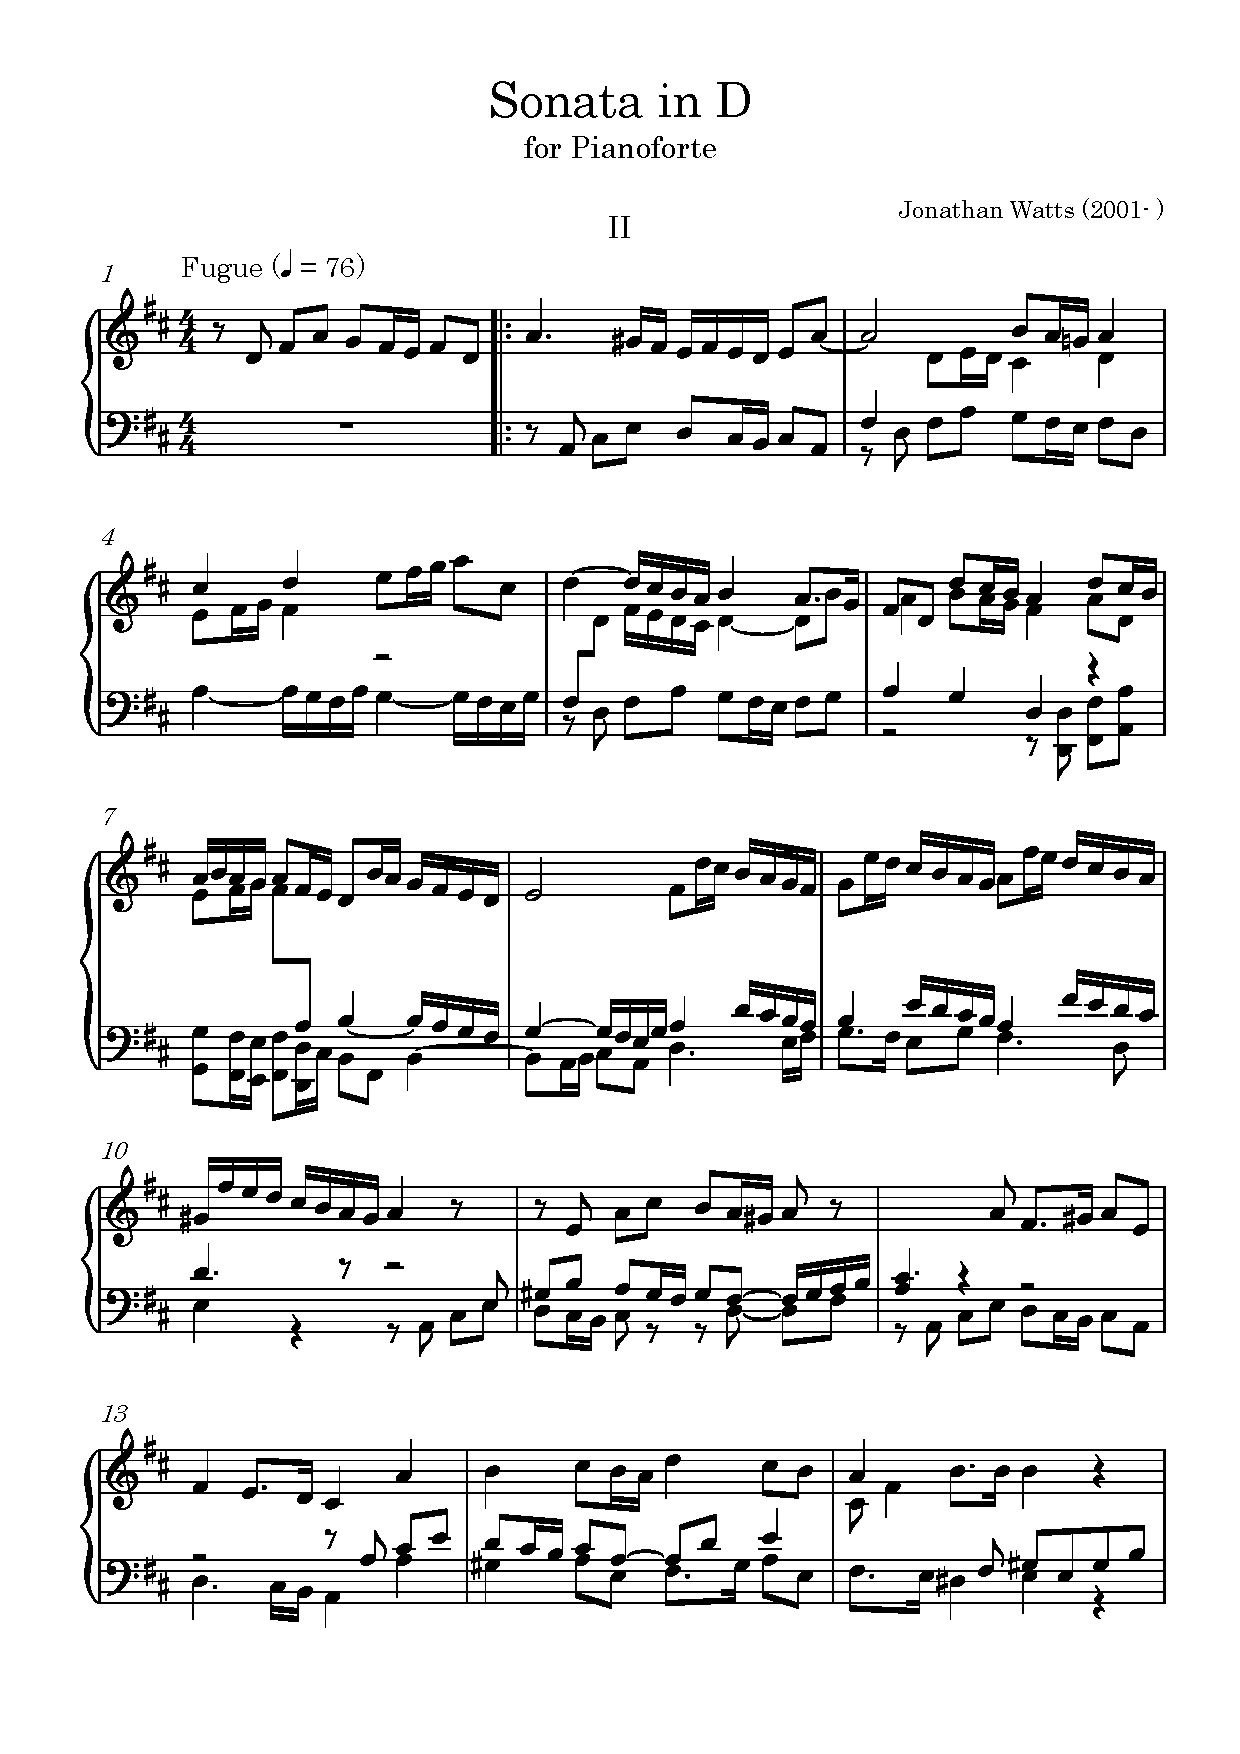
\includepdf[pages=-,pagecommand={},width=\textwidth]{sonata2.pdf}
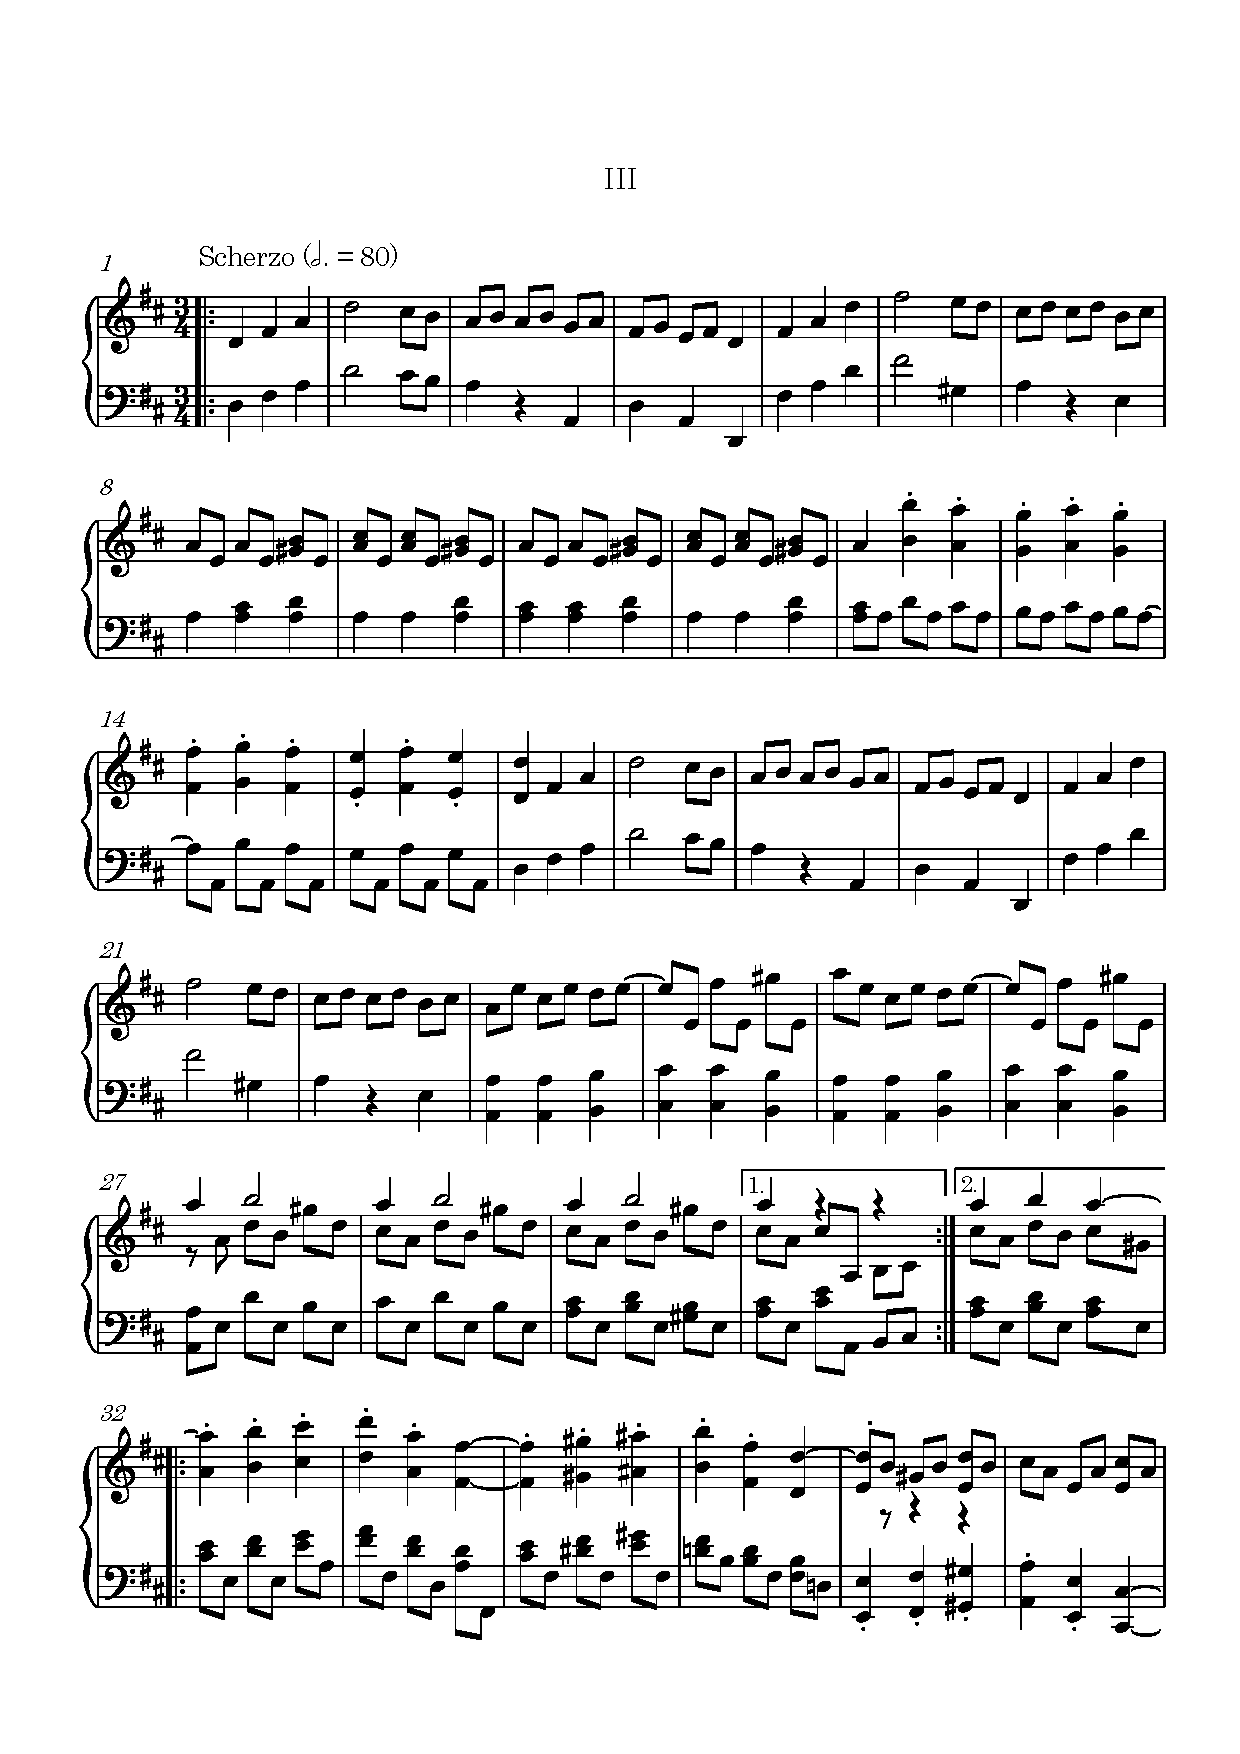
\includepdf[pages=-,pagecommand={},width=\textwidth]{sonata3.pdf}
\clearpage

\setlength{\voffset}{-1in}

\pagestyle{fancy}

\chapter{Puzzles---GNU Sudoku}

\centering

\pagestyle{empty}

\vspace{\fill}
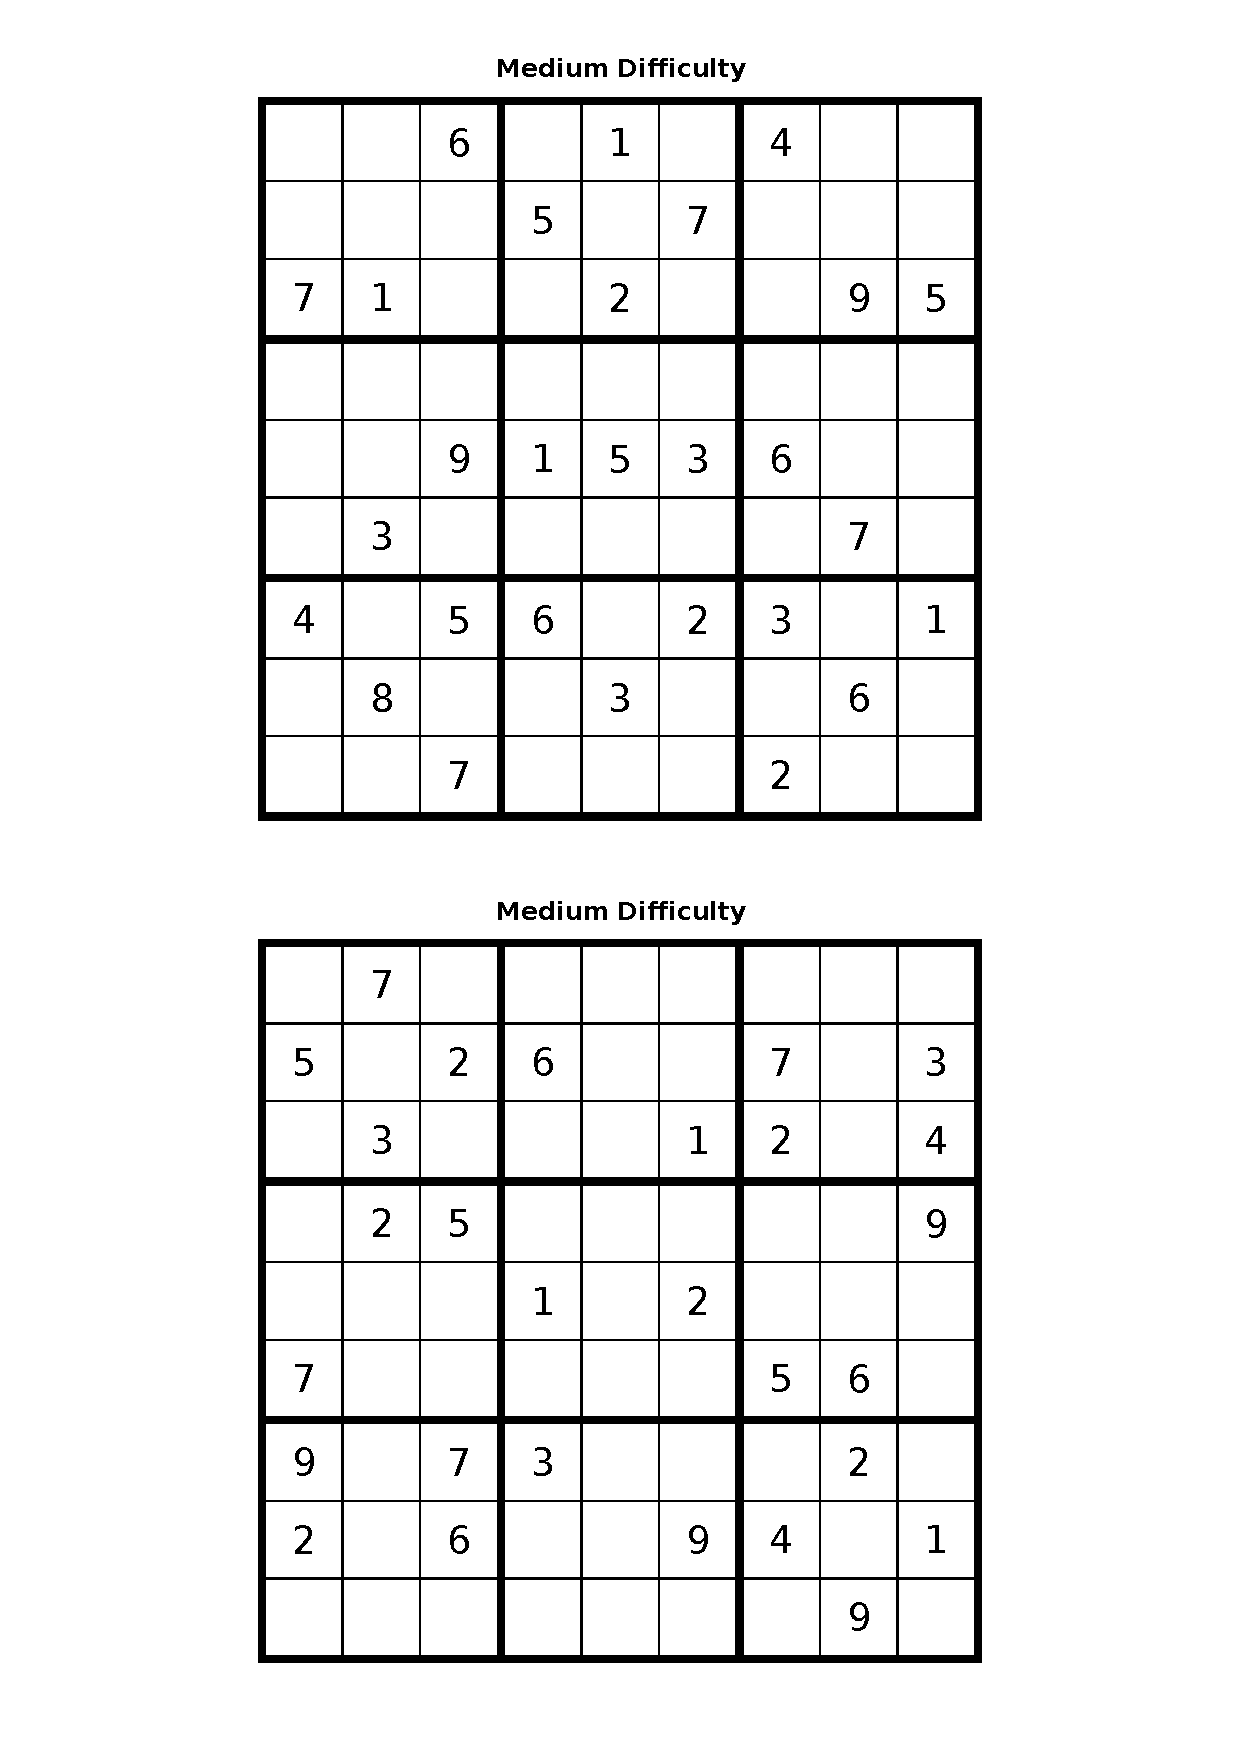
\includegraphics[height=24cm]{easy.pdf}
\vspace{\fill}

\vspace{\fill}
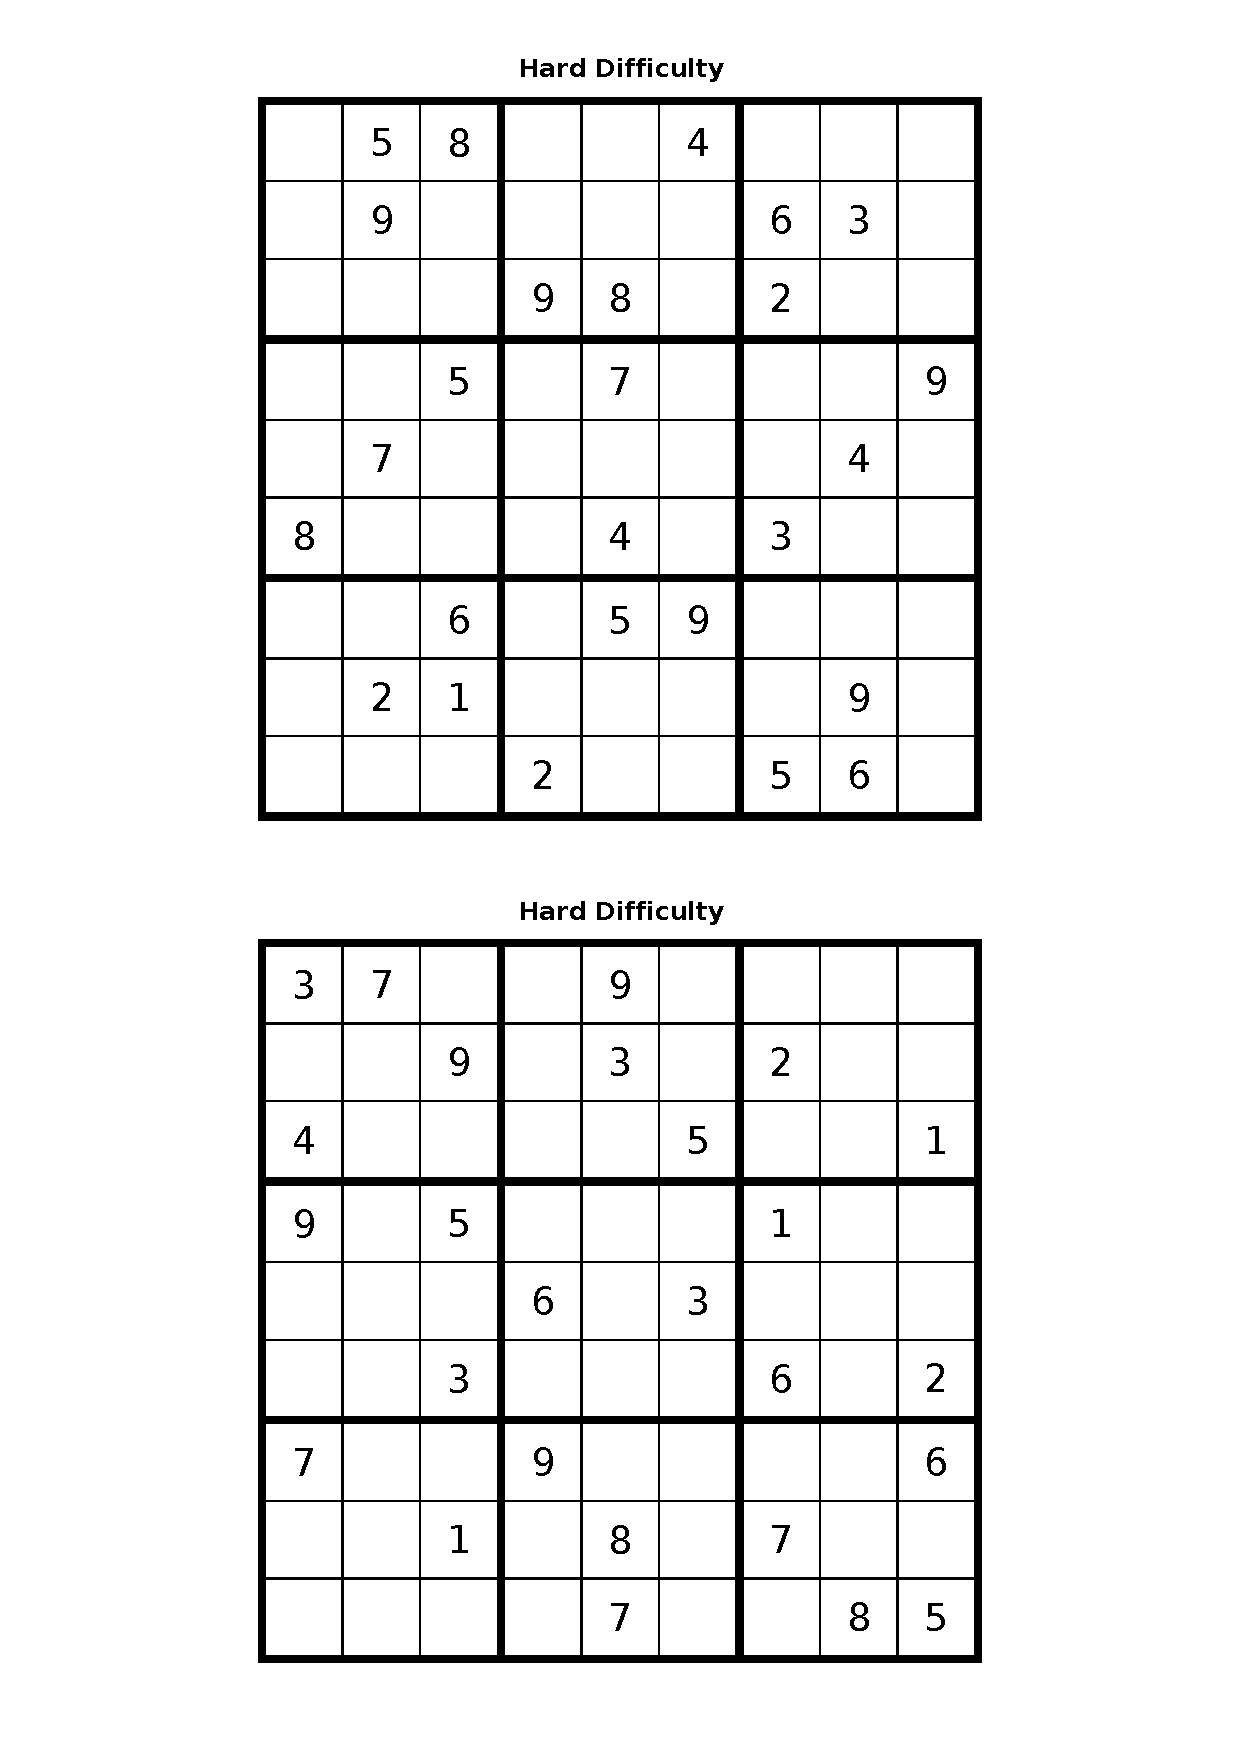
\includegraphics[height=24cm]{hard.pdf}
\vspace{\fill}

\vspace{\fill}
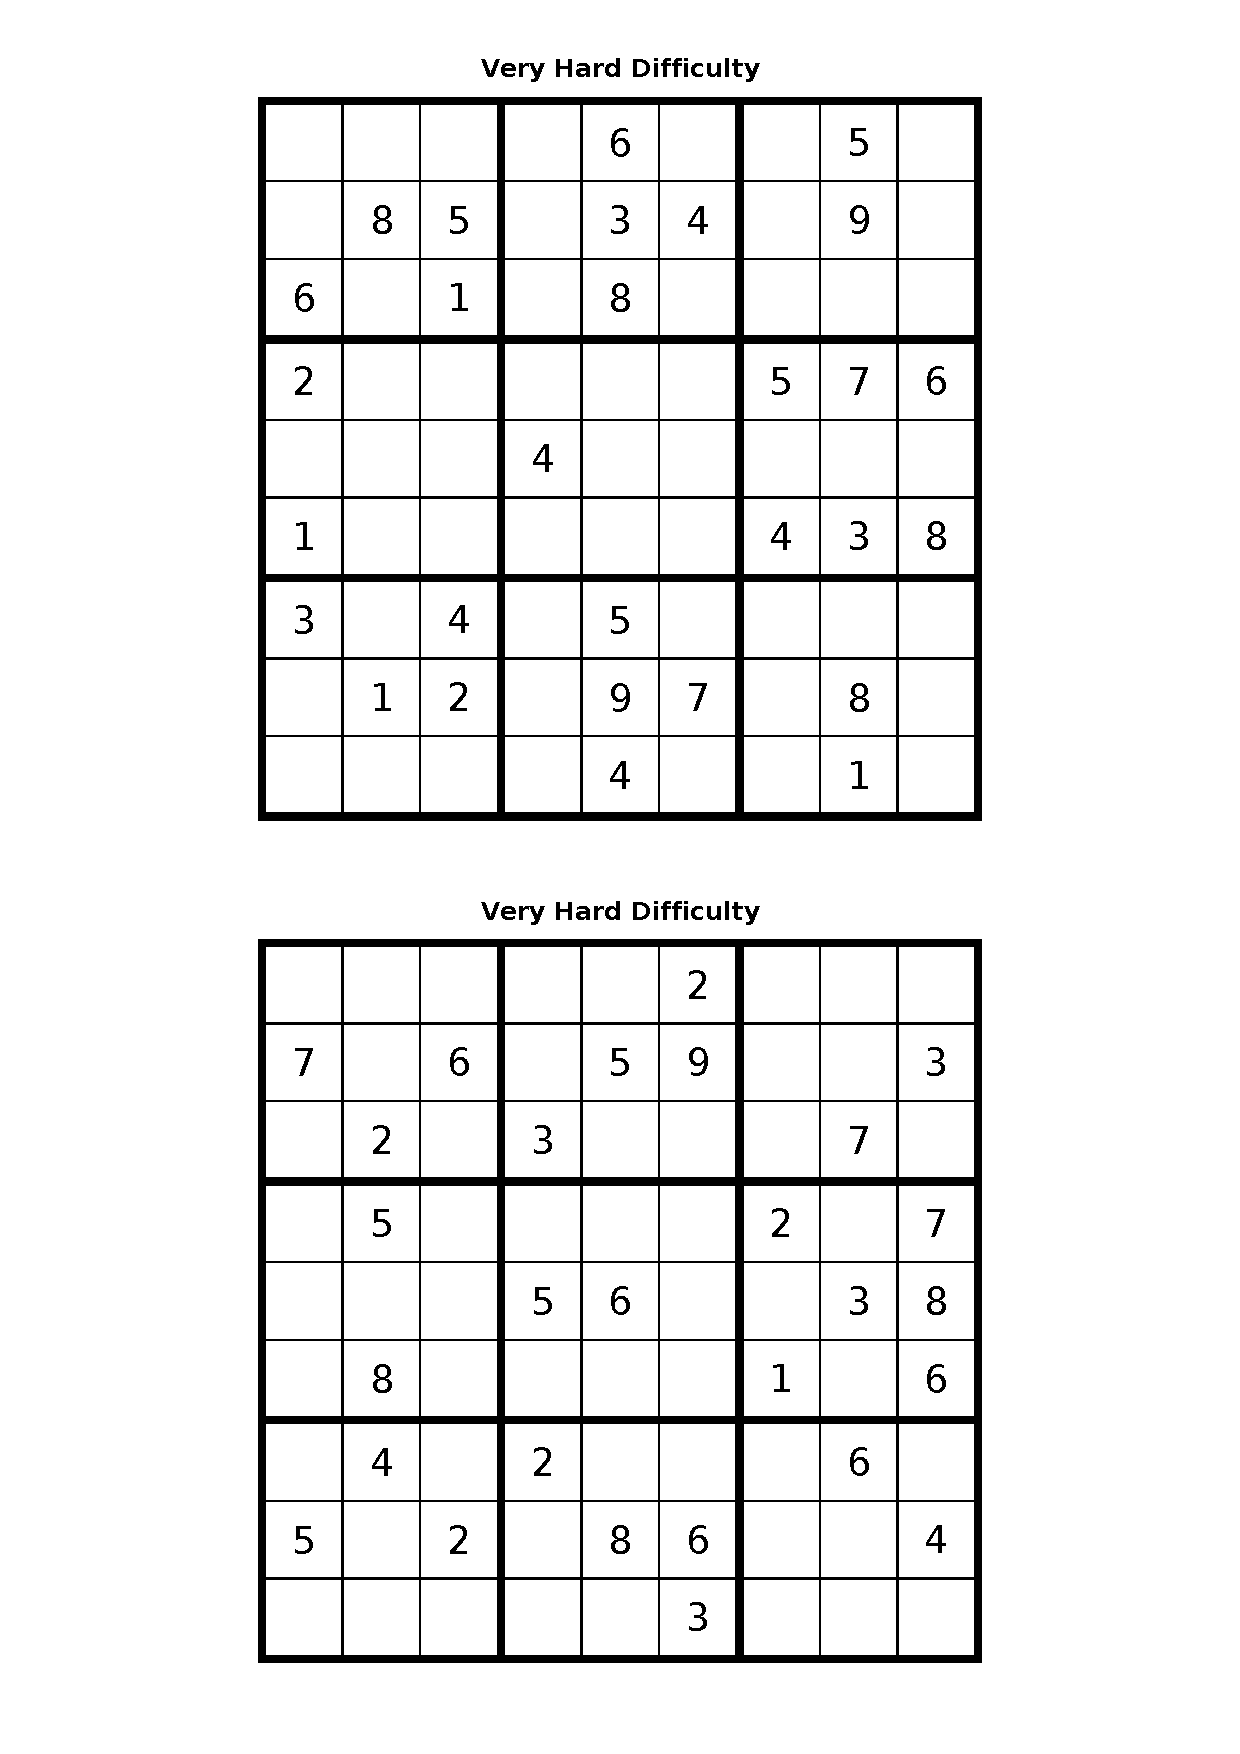
\includegraphics[height=24cm]{veryhard.pdf}
\vspace{\fill}

\clearpage

\pagestyle{empty}
\setlength{\parskip}{0em}
\centering


\includegraphics[width=0.3\textwidth]{logo.png}

\vspace{3em}

\Huge

\textbf{Westminster School Library Committee}

\Large

\vspace{1em}

\textbf{\textit{Dedicated to the betterment of the Library.}}

\vspace{1.5em}

\hrule

\vspace{1.5em}

\huge

The Library

\Large

\begin{paracol}{2}

\begin{flushright}

\textbf{Librarian}

\textbf{Deputy Librarian}

\textbf{Library Assistants}

\textbf{Chairperson}

\textbf{Assistant Chairperson}

\textbf{Editor}

\end{flushright}

\switchcolumn

\begin{flushleft}

\vspace{0.05em}

Mrs Goetzee

Ms Stone

Ms Stringer and M\textsuperscript{me} Dessouroux

Jonny Heywood

Isky Mathews

Joshua Loo

\end{flushleft}

\end{paracol}

\huge

Members of the Committee

\Large

\begin{paracol}{2}

\begin{flushright}
Adam Mee

Anna Yang

Anshu Banerjee

Arjun Seth

Ben Goodrick-Green

Ben Weiss

Benedict Mee

Benedict Randall Shaw

Brandon Tang

Isky Mathews

Jadd Virji

James Bithell

\end{flushright}

\switchcolumn

\begin{flushleft}
Jonathan Watts

Jonny Heywood

Joshua Loo

Joshua Rosen

Lorna Bo

Margaret Teh

Michelle Yang

Morayo Adesina

Polina Zakharov

Robert Doane-Solomon

Shri Lekkala

Thomas Adamo
\end{flushleft}

\end{paracol}

\end{document}